% Options for packages loaded elsewhere
\PassOptionsToPackage{unicode}{hyperref}
\PassOptionsToPackage{hyphens}{url}
%
\documentclass[
  12pt,
]{article}
\usepackage{amsmath,amssymb}
\usepackage{iftex}
\ifPDFTeX
  \usepackage[T1]{fontenc}
  \usepackage[utf8]{inputenc}
  \usepackage{textcomp} % provide euro and other symbols
\else % if luatex or xetex
  \usepackage{unicode-math} % this also loads fontspec
  \defaultfontfeatures{Scale=MatchLowercase}
  \defaultfontfeatures[\rmfamily]{Ligatures=TeX,Scale=1}
\fi
\usepackage{lmodern}
\ifPDFTeX\else
  % xetex/luatex font selection
\fi
% Use upquote if available, for straight quotes in verbatim environments
\IfFileExists{upquote.sty}{\usepackage{upquote}}{}
\IfFileExists{microtype.sty}{% use microtype if available
  \usepackage[]{microtype}
  \UseMicrotypeSet[protrusion]{basicmath} % disable protrusion for tt fonts
}{}
\makeatletter
\@ifundefined{KOMAClassName}{% if non-KOMA class
  \IfFileExists{parskip.sty}{%
    \usepackage{parskip}
  }{% else
    \setlength{\parindent}{0pt}
    \setlength{\parskip}{6pt plus 2pt minus 1pt}}
}{% if KOMA class
  \KOMAoptions{parskip=half}}
\makeatother
\usepackage{xcolor}
\usepackage[margin=1in]{geometry}
\usepackage{color}
\usepackage{fancyvrb}
\newcommand{\VerbBar}{|}
\newcommand{\VERB}{\Verb[commandchars=\\\{\}]}
\DefineVerbatimEnvironment{Highlighting}{Verbatim}{commandchars=\\\{\}}
% Add ',fontsize=\small' for more characters per line
\usepackage{framed}
\definecolor{shadecolor}{RGB}{248,248,248}
\newenvironment{Shaded}{\begin{snugshade}}{\end{snugshade}}
\newcommand{\AlertTok}[1]{\textcolor[rgb]{0.94,0.16,0.16}{#1}}
\newcommand{\AnnotationTok}[1]{\textcolor[rgb]{0.56,0.35,0.01}{\textbf{\textit{#1}}}}
\newcommand{\AttributeTok}[1]{\textcolor[rgb]{0.13,0.29,0.53}{#1}}
\newcommand{\BaseNTok}[1]{\textcolor[rgb]{0.00,0.00,0.81}{#1}}
\newcommand{\BuiltInTok}[1]{#1}
\newcommand{\CharTok}[1]{\textcolor[rgb]{0.31,0.60,0.02}{#1}}
\newcommand{\CommentTok}[1]{\textcolor[rgb]{0.56,0.35,0.01}{\textit{#1}}}
\newcommand{\CommentVarTok}[1]{\textcolor[rgb]{0.56,0.35,0.01}{\textbf{\textit{#1}}}}
\newcommand{\ConstantTok}[1]{\textcolor[rgb]{0.56,0.35,0.01}{#1}}
\newcommand{\ControlFlowTok}[1]{\textcolor[rgb]{0.13,0.29,0.53}{\textbf{#1}}}
\newcommand{\DataTypeTok}[1]{\textcolor[rgb]{0.13,0.29,0.53}{#1}}
\newcommand{\DecValTok}[1]{\textcolor[rgb]{0.00,0.00,0.81}{#1}}
\newcommand{\DocumentationTok}[1]{\textcolor[rgb]{0.56,0.35,0.01}{\textbf{\textit{#1}}}}
\newcommand{\ErrorTok}[1]{\textcolor[rgb]{0.64,0.00,0.00}{\textbf{#1}}}
\newcommand{\ExtensionTok}[1]{#1}
\newcommand{\FloatTok}[1]{\textcolor[rgb]{0.00,0.00,0.81}{#1}}
\newcommand{\FunctionTok}[1]{\textcolor[rgb]{0.13,0.29,0.53}{\textbf{#1}}}
\newcommand{\ImportTok}[1]{#1}
\newcommand{\InformationTok}[1]{\textcolor[rgb]{0.56,0.35,0.01}{\textbf{\textit{#1}}}}
\newcommand{\KeywordTok}[1]{\textcolor[rgb]{0.13,0.29,0.53}{\textbf{#1}}}
\newcommand{\NormalTok}[1]{#1}
\newcommand{\OperatorTok}[1]{\textcolor[rgb]{0.81,0.36,0.00}{\textbf{#1}}}
\newcommand{\OtherTok}[1]{\textcolor[rgb]{0.56,0.35,0.01}{#1}}
\newcommand{\PreprocessorTok}[1]{\textcolor[rgb]{0.56,0.35,0.01}{\textit{#1}}}
\newcommand{\RegionMarkerTok}[1]{#1}
\newcommand{\SpecialCharTok}[1]{\textcolor[rgb]{0.81,0.36,0.00}{\textbf{#1}}}
\newcommand{\SpecialStringTok}[1]{\textcolor[rgb]{0.31,0.60,0.02}{#1}}
\newcommand{\StringTok}[1]{\textcolor[rgb]{0.31,0.60,0.02}{#1}}
\newcommand{\VariableTok}[1]{\textcolor[rgb]{0.00,0.00,0.00}{#1}}
\newcommand{\VerbatimStringTok}[1]{\textcolor[rgb]{0.31,0.60,0.02}{#1}}
\newcommand{\WarningTok}[1]{\textcolor[rgb]{0.56,0.35,0.01}{\textbf{\textit{#1}}}}
\usepackage{longtable,booktabs,array}
\usepackage{calc} % for calculating minipage widths
% Correct order of tables after \paragraph or \subparagraph
\usepackage{etoolbox}
\makeatletter
\patchcmd\longtable{\par}{\if@noskipsec\mbox{}\fi\par}{}{}
\makeatother
% Allow footnotes in longtable head/foot
\IfFileExists{footnotehyper.sty}{\usepackage{footnotehyper}}{\usepackage{footnote}}
\makesavenoteenv{longtable}
\usepackage{graphicx}
\makeatletter
\def\maxwidth{\ifdim\Gin@nat@width>\linewidth\linewidth\else\Gin@nat@width\fi}
\def\maxheight{\ifdim\Gin@nat@height>\textheight\textheight\else\Gin@nat@height\fi}
\makeatother
% Scale images if necessary, so that they will not overflow the page
% margins by default, and it is still possible to overwrite the defaults
% using explicit options in \includegraphics[width, height, ...]{}
\setkeys{Gin}{width=\maxwidth,height=\maxheight,keepaspectratio}
% Set default figure placement to htbp
\makeatletter
\def\fps@figure{htbp}
\makeatother
\setlength{\emergencystretch}{3em} % prevent overfull lines
\providecommand{\tightlist}{%
  \setlength{\itemsep}{0pt}\setlength{\parskip}{0pt}}
\setcounter{secnumdepth}{-\maxdimen} % remove section numbering
% definitions for citeproc citations
\NewDocumentCommand\citeproctext{}{}
\NewDocumentCommand\citeproc{mm}{%
  \begingroup\def\citeproctext{#2}\cite{#1}\endgroup}
\makeatletter
 % allow citations to break across lines
 \let\@cite@ofmt\@firstofone
 % avoid brackets around text for \cite:
 \def\@biblabel#1{}
 \def\@cite#1#2{{#1\if@tempswa , #2\fi}}
\makeatother
\newlength{\cslhangindent}
\setlength{\cslhangindent}{1.5em}
\newlength{\csllabelwidth}
\setlength{\csllabelwidth}{3em}
\newenvironment{CSLReferences}[2] % #1 hanging-indent, #2 entry-spacing
 {\begin{list}{}{%
  \setlength{\itemindent}{0pt}
  \setlength{\leftmargin}{0pt}
  \setlength{\parsep}{0pt}
  % turn on hanging indent if param 1 is 1
  \ifodd #1
   \setlength{\leftmargin}{\cslhangindent}
   \setlength{\itemindent}{-1\cslhangindent}
  \fi
  % set entry spacing
  \setlength{\itemsep}{#2\baselineskip}}}
 {\end{list}}
\usepackage{calc}
\newcommand{\CSLBlock}[1]{\hfill\break\parbox[t]{\linewidth}{\strut\ignorespaces#1\strut}}
\newcommand{\CSLLeftMargin}[1]{\parbox[t]{\csllabelwidth}{\strut#1\strut}}
\newcommand{\CSLRightInline}[1]{\parbox[t]{\linewidth - \csllabelwidth}{\strut#1\strut}}
\newcommand{\CSLIndent}[1]{\hspace{\cslhangindent}#1}
\usepackage{setspace}
\onehalfspacing
\usepackage{etoolbox}
\usepackage{float}
\usepackage{graphicx}
\usepackage{fvextra}
\ifLuaTeX
  \usepackage{selnolig}  % disable illegal ligatures
\fi
\usepackage{bookmark}
\IfFileExists{xurl.sty}{\usepackage{xurl}}{} % add URL line breaks if available
\urlstyle{same}
\hypersetup{
  hidelinks,
  pdfcreator={LaTeX via pandoc}}

\author{}
\date{\vspace{-2.5em}}

\begin{document}

\section{Appendix B : Code}\label{appendix-b-code}

Coding for this section was completed using RStudio 2024.09.0+375
(``Cranberry Hibiscus'' Release) and was based on R and MATLAB code
provided by Professor Tim Gebbie(STA4028Z).

\subsubsection{2.1 Libraries (Gebbie, 2025d)}\label{libraries-tim_prep}

\begin{Shaded}
\begin{Highlighting}[]
\CommentTok{\# load required libraries}
\FunctionTok{suppressPackageStartupMessages}\NormalTok{(\{}
\FunctionTok{library}\NormalTok{(openxlsx)     }
\FunctionTok{library}\NormalTok{(timeSeries)   }
\FunctionTok{library}\NormalTok{(xts)          }
\FunctionTok{library}\NormalTok{(zoo)          }
\FunctionTok{library}\NormalTok{(matrixStats) }
\FunctionTok{library}\NormalTok{(quadprog)     }
\FunctionTok{library}\NormalTok{(knitr)        }
\FunctionTok{library}\NormalTok{(dplyr)        }
\FunctionTok{library}\NormalTok{(ggplot2)      }
\FunctionTok{library}\NormalTok{(tidyr)  }
\FunctionTok{library}\NormalTok{(PerformanceAnalytics)}
\NormalTok{\})}
\end{Highlighting}
\end{Shaded}

\subsubsection{2.2 Load data and preprocessing (Gebbie,
2025d)}\label{load-data-and-preprocessing-tim_prep}

\begin{Shaded}
\begin{Highlighting}[]
\CommentTok{\# reading in all 4 sheets into a list}
\NormalTok{dfS }\OtherTok{\textless{}{-}} \FunctionTok{list}\NormalTok{()}
\ControlFlowTok{for}\NormalTok{ (i }\ControlFlowTok{in} \DecValTok{1}\SpecialCharTok{:}\DecValTok{4}\NormalTok{) \{}
\NormalTok{  dfS[[i]] }\OtherTok{\textless{}{-}} \FunctionTok{read.xlsx}\NormalTok{(}\StringTok{"\_raw\_data/PT{-}TAA{-}JSE{-}Daily{-}1994{-}2017.xlsx"}\NormalTok{, }\AttributeTok{sheet =}\NormalTok{ i, }\AttributeTok{detectDates =} \ConstantTok{TRUE}\NormalTok{)}
  \FunctionTok{cat}\NormalTok{(}\StringTok{"Sheet"}\NormalTok{, i, }\StringTok{"loaded with dimensions:"}\NormalTok{, }\FunctionTok{dim}\NormalTok{(dfS[[i]]), }\StringTok{"}\SpecialCharTok{\textbackslash{}n}\StringTok{"}\NormalTok{)}
\NormalTok{\}}
\end{Highlighting}
\end{Shaded}

\begin{verbatim}
## Sheet 1 loaded with dimensions: 8439 2 
## Sheet 2 loaded with dimensions: 8405 4 
## Sheet 3 loaded with dimensions: 8439 28 
## Sheet 4 loaded with dimensions: 8439 20
\end{verbatim}

\begin{Shaded}
\begin{Highlighting}[]
\CommentTok{\# define entities and which assets to keep}
\NormalTok{Entities }\OtherTok{\textless{}{-}} \FunctionTok{c}\NormalTok{(}\StringTok{\textquotesingle{}X1\textquotesingle{}}\NormalTok{,}\StringTok{\textquotesingle{}STEFI\textquotesingle{}}\NormalTok{,}\StringTok{\textquotesingle{}ALBI\textquotesingle{}}\NormalTok{,}\StringTok{\textquotesingle{}J203\textquotesingle{}}\NormalTok{,}\StringTok{\textquotesingle{}J500\textquotesingle{}}\NormalTok{, }\FunctionTok{sprintf}\NormalTok{(}\StringTok{"J5\%d"}\NormalTok{, }\FunctionTok{seq}\NormalTok{(}\DecValTok{10}\NormalTok{,}\DecValTok{90}\NormalTok{,}\AttributeTok{by=}\DecValTok{10}\NormalTok{)))}
\NormalTok{Items    }\OtherTok{\textless{}{-}} \FunctionTok{c}\NormalTok{(}\StringTok{\textquotesingle{}Date\textquotesingle{}}\NormalTok{,}\StringTok{\textquotesingle{}TRI\textquotesingle{}}\NormalTok{,}\StringTok{\textquotesingle{}Stefi\textquotesingle{}}\NormalTok{)}

\CommentTok{\#cleaning each sheet}
\ControlFlowTok{for}\NormalTok{ (i }\ControlFlowTok{in} \DecValTok{1}\SpecialCharTok{:}\DecValTok{4}\NormalTok{) \{}
\NormalTok{  tI0 }\OtherTok{\textless{}{-}} \FunctionTok{sapply}\NormalTok{(}\FunctionTok{colnames}\NormalTok{(dfS[[i]]), }\ControlFlowTok{function}\NormalTok{(x) }\FunctionTok{any}\NormalTok{(}\FunctionTok{grepl}\NormalTok{(}\FunctionTok{paste}\NormalTok{(Entities, }\AttributeTok{collapse=}\StringTok{"|"}\NormalTok{), x)))}
\NormalTok{  tI1 }\OtherTok{\textless{}{-}} \FunctionTok{sapply}\NormalTok{(dfS[[i]][}\DecValTok{2}\NormalTok{,], }\ControlFlowTok{function}\NormalTok{(x) }\FunctionTok{any}\NormalTok{(}\FunctionTok{grepl}\NormalTok{(}\FunctionTok{paste}\NormalTok{(Items, }\AttributeTok{collapse=}\StringTok{"|"}\NormalTok{), x)))}
\NormalTok{  tI  }\OtherTok{\textless{}{-}}\NormalTok{ tI0 }\SpecialCharTok{\&}\NormalTok{ tI1}
  
  \CommentTok{\# remove header rows}
\NormalTok{  dfS[[i]] }\OtherTok{\textless{}{-}}\NormalTok{ dfS[[i]][}\SpecialCharTok{{-}}\FunctionTok{c}\NormalTok{(}\DecValTok{1}\NormalTok{,}\DecValTok{2}\NormalTok{), tI]}
  \FunctionTok{names}\NormalTok{(dfS[[i]])[}\DecValTok{1}\NormalTok{] }\OtherTok{\textless{}{-}} \StringTok{"Date"}
  
\NormalTok{  newColNames }\OtherTok{\textless{}{-}} \FunctionTok{strsplit}\NormalTok{(}\FunctionTok{colnames}\NormalTok{(dfS[[i]]), }\StringTok{":"}\NormalTok{)}
  \ControlFlowTok{for}\NormalTok{(m }\ControlFlowTok{in} \DecValTok{2}\SpecialCharTok{:}\FunctionTok{length}\NormalTok{(newColNames)) }\FunctionTok{names}\NormalTok{(dfS[[i]])[m] }\OtherTok{\textless{}{-}}\NormalTok{ newColNames[[m]][}\DecValTok{1}\NormalTok{]}
  
  \FunctionTok{cat}\NormalTok{(}\StringTok{"Sheet"}\NormalTok{, i, }\StringTok{"columns after cleaning:"}\NormalTok{, }\FunctionTok{colnames}\NormalTok{(dfS[[i]]), }\StringTok{"}\SpecialCharTok{\textbackslash{}n}\StringTok{"}\NormalTok{)}
\NormalTok{\}}
\end{Highlighting}
\end{Shaded}

\begin{verbatim}
## Sheet 1 columns after cleaning: Date ALBI 
## Sheet 2 columns after cleaning: Date RATESTEFI 
## Sheet 3 columns after cleaning: Date J500 J510 J520 J530 J540 J550 J560 J580 J590 
## Sheet 4 columns after cleaning: Date J203
\end{verbatim}

\begin{Shaded}
\begin{Highlighting}[]
\CommentTok{\# fixing ALBI column}
\NormalTok{dfS[[}\DecValTok{1}\NormalTok{]][,}\DecValTok{2}\NormalTok{] }\OtherTok{\textless{}{-}} \FunctionTok{as.numeric}\NormalTok{(dfS[[}\DecValTok{1}\NormalTok{]][,}\DecValTok{2}\NormalTok{])  }
\NormalTok{dfS[[}\DecValTok{1}\NormalTok{]] }\OtherTok{\textless{}{-}}\NormalTok{ dfS[[}\DecValTok{1}\NormalTok{]][}\SpecialCharTok{!}\FunctionTok{is.na}\NormalTok{(dfS[[}\DecValTok{1}\NormalTok{]][,}\DecValTok{2}\NormalTok{]), ]}\CommentTok{\#removes rows where ALBI is NA}
\end{Highlighting}
\end{Shaded}

\subsubsection{2.3 Merge into single timeSeries object (Gebbie,
2025d)}\label{merge-into-single-timeseries-object-tim_prep}

\begin{Shaded}
\begin{Highlighting}[]
\CommentTok{\# converts first sheet to timeSeries}
\NormalTok{tsTAA }\OtherTok{\textless{}{-}} \FunctionTok{timeSeries}\NormalTok{(dfS[[}\DecValTok{1}\NormalTok{]][, }\DecValTok{2}\SpecialCharTok{:}\FunctionTok{ncol}\NormalTok{(dfS[[}\DecValTok{1}\NormalTok{]])], }\FunctionTok{as.Date}\NormalTok{(dfS[[}\DecValTok{1}\NormalTok{]][,}\DecValTok{1}\NormalTok{]))}
\FunctionTok{cat}\NormalTok{(}\StringTok{"Initial tsTAA dimensions:"}\NormalTok{, }\FunctionTok{dim}\NormalTok{(tsTAA), }\StringTok{"}\SpecialCharTok{\textbackslash{}n}\StringTok{"}\NormalTok{)}
\end{Highlighting}
\end{Shaded}

\begin{verbatim}
## Initial tsTAA dimensions: 4324 1
\end{verbatim}

\begin{Shaded}
\begin{Highlighting}[]
\CommentTok{\# merges remaining sheets}
\ControlFlowTok{for}\NormalTok{ (i }\ControlFlowTok{in} \DecValTok{2}\SpecialCharTok{:}\DecValTok{4}\NormalTok{) \{}
\NormalTok{  tsTmp }\OtherTok{\textless{}{-}} \FunctionTok{timeSeries}\NormalTok{(dfS[[i]][, }\DecValTok{2}\SpecialCharTok{:}\FunctionTok{ncol}\NormalTok{(dfS[[i]])], }\FunctionTok{as.Date}\NormalTok{(dfS[[i]][,}\DecValTok{1}\NormalTok{]))}
\NormalTok{  tsTAA }\OtherTok{\textless{}{-}} \FunctionTok{cbind}\NormalTok{(tsTAA, tsTmp)}
  \FunctionTok{cat}\NormalTok{(}\StringTok{"After merging sheet"}\NormalTok{, i, }\StringTok{"dimensions:"}\NormalTok{, }\FunctionTok{dim}\NormalTok{(tsTAA), }\StringTok{"}\SpecialCharTok{\textbackslash{}n}\StringTok{"}\NormalTok{)}
\NormalTok{\}}
\end{Highlighting}
\end{Shaded}

\begin{verbatim}
## After merging sheet 2 dimensions: 8437 2 
## After merging sheet 3 dimensions: 8437 11 
## After merging sheet 4 dimensions: 8437 12
\end{verbatim}

\begin{Shaded}
\begin{Highlighting}[]
\CommentTok{\# renaming indices for clarity}
\FunctionTok{setFinCenter}\NormalTok{(tsTAA) }\OtherTok{\textless{}{-}} \StringTok{"Johannesburg"}
\FunctionTok{names}\NormalTok{(tsTAA)[}\FunctionTok{grep}\NormalTok{(}\StringTok{"TS.1.1"}\NormalTok{, }\FunctionTok{names}\NormalTok{(tsTAA))] }\OtherTok{\textless{}{-}} \StringTok{"ALBI"}
\FunctionTok{names}\NormalTok{(tsTAA)[}\FunctionTok{grep}\NormalTok{(}\StringTok{"TS.1.2"}\NormalTok{, }\FunctionTok{names}\NormalTok{(tsTAA))] }\OtherTok{\textless{}{-}} \StringTok{"STEFI"}
\FunctionTok{names}\NormalTok{(tsTAA)[}\FunctionTok{grep}\NormalTok{(}\StringTok{"TS.1"}\NormalTok{, }\FunctionTok{names}\NormalTok{(tsTAA))] }\OtherTok{\textless{}{-}} \StringTok{"ALSI"}

\FunctionTok{cat}\NormalTok{(}\StringTok{"Columns after renaming:"}\NormalTok{, }\FunctionTok{colnames}\NormalTok{(tsTAA), }\StringTok{"}\SpecialCharTok{\textbackslash{}n}\StringTok{"}\NormalTok{)}
\end{Highlighting}
\end{Shaded}

\begin{verbatim}
## Columns after renaming: ALBI STEFI J500 J510 J520 J530 J540 J550 J560 J580 J590 ALSI
\end{verbatim}

\begin{Shaded}
\begin{Highlighting}[]
\CommentTok{\#all numeric columns are numeric}
\ControlFlowTok{for}\NormalTok{ (j }\ControlFlowTok{in} \DecValTok{1}\SpecialCharTok{:}\FunctionTok{ncol}\NormalTok{(tsTAA)) \{}
\NormalTok{  tsTAA[, j] }\OtherTok{\textless{}{-}} \FunctionTok{as.numeric}\NormalTok{(tsTAA[, j])}
\NormalTok{\}}
\CommentTok{\#remove rows with all NAs}
\NormalTok{tsTAA }\OtherTok{\textless{}{-}}\NormalTok{ tsTAA[}\FunctionTok{rowSums}\NormalTok{(}\FunctionTok{is.na}\NormalTok{(tsTAA)) }\SpecialCharTok{\textless{}} \FunctionTok{ncol}\NormalTok{(tsTAA), ]}

\CommentTok{\# Using timeSeries daily2monthly and ensure tsTAA is valid}
\NormalTok{tsTAA\_monthly }\OtherTok{\textless{}{-}} \FunctionTok{tryCatch}\NormalTok{(}
  \FunctionTok{daily2monthly}\NormalTok{(tsTAA),}
  \AttributeTok{error =} \ControlFlowTok{function}\NormalTok{(e) \{}
    \FunctionTok{stop}\NormalTok{(}\StringTok{"Error in daily2monthly: tsTAA might contain non{-}timeSeries columns or non{-}numeric values"}\NormalTok{)}
\NormalTok{  \}}
\NormalTok{)}

\CommentTok{\#  monthly price index}
\NormalTok{tsIdx  }\OtherTok{\textless{}{-}} \FunctionTok{index2wealth}\NormalTok{(tsTAA\_monthly)}

\CommentTok{\# geometric monthly returns}
\NormalTok{tsGRet }\OtherTok{\textless{}{-}} \FunctionTok{diff}\NormalTok{(}\FunctionTok{log}\NormalTok{(tsIdx))}

\FunctionTok{cat}\NormalTok{(}\StringTok{"tsTAA\_monthly dimensions:"}\NormalTok{, }\FunctionTok{dim}\NormalTok{(tsTAA\_monthly), }\StringTok{"}\SpecialCharTok{\textbackslash{}n}\StringTok{"}\NormalTok{)}
\end{Highlighting}
\end{Shaded}

\begin{verbatim}
## tsTAA_monthly dimensions: 261 12
\end{verbatim}

\begin{Shaded}
\begin{Highlighting}[]
\FunctionTok{cat}\NormalTok{(}\StringTok{"tsGRet dimensions:"}\NormalTok{, }\FunctionTok{dim}\NormalTok{(tsGRet), }\StringTok{"}\SpecialCharTok{\textbackslash{}n}\StringTok{"}\NormalTok{)}
\end{Highlighting}
\end{Shaded}

\begin{verbatim}
## tsGRet dimensions: 261 12
\end{verbatim}

\begin{Shaded}
\begin{Highlighting}[]
\FunctionTok{cat}\NormalTok{(}\StringTok{"Columns in tsGRet:}\SpecialCharTok{\textbackslash{}n}\StringTok{"}\NormalTok{); }\FunctionTok{print}\NormalTok{(}\FunctionTok{colnames}\NormalTok{(tsGRet))}
\end{Highlighting}
\end{Shaded}

\begin{verbatim}
## Columns in tsGRet:
\end{verbatim}

\begin{verbatim}
##  [1] "ALBI"  "STEFI" "J500"  "J510"  "J520"  "J530"  "J540"  "J550"  "J560" 
## [10] "J580"  "J590"  "ALSI"
\end{verbatim}

\subsubsection{2.4 Arithmetic Returns (Gebbie,
2025c)}\label{arithmetic-returns-tim_btmlx}

\begin{Shaded}
\begin{Highlighting}[]
\FunctionTok{setFinCenter}\NormalTok{(tsTAA) }\OtherTok{\textless{}{-}} \StringTok{"Africa/Johannesburg"}
\FunctionTok{summary}\NormalTok{(dfS[[}\DecValTok{1}\NormalTok{]][,}\DecValTok{2}\NormalTok{])}
\end{Highlighting}
\end{Shaded}

\begin{verbatim}
##    Min. 1st Qu.  Median    Mean 3rd Qu.    Max. 
##   173.7   256.9   343.9   357.5   442.0   545.9
\end{verbatim}

\begin{Shaded}
\begin{Highlighting}[]
\CommentTok{\# Checks that tsTAA is a proper \textquotesingle{}timeSeries\textquotesingle{} object}
\NormalTok{tsTAA\_monthly }\OtherTok{\textless{}{-}} \FunctionTok{tryCatch}\NormalTok{(}
  \FunctionTok{daily2monthly}\NormalTok{(tsTAA),}
  \AttributeTok{error =} \ControlFlowTok{function}\NormalTok{(e) \{}
    \FunctionTok{message}\NormalTok{(}\StringTok{"Error in daily2monthly(): converting tsTAA to xts first"}\NormalTok{)}
\NormalTok{    xts\_obj }\OtherTok{\textless{}{-}} \FunctionTok{as.xts}\NormalTok{(tsTAA)}
    \FunctionTok{apply.monthly}\NormalTok{(xts\_obj, colMeans, }\AttributeTok{na.rm=}\ConstantTok{TRUE}\NormalTok{)}
\NormalTok{  \}}
\NormalTok{)}



\CommentTok{\#geometric returns}
\NormalTok{tsGRet }\OtherTok{\textless{}{-}} \FunctionTok{diff}\NormalTok{(}\FunctionTok{log}\NormalTok{(tsTAA\_monthly))}

\CommentTok{\#  fill missing data using LOCF}
\NormalTok{tsGRet\_filled }\OtherTok{\textless{}{-}} \FunctionTok{na.locf}\NormalTok{(}\FunctionTok{as.xts}\NormalTok{(tsGRet), }\AttributeTok{na.rm =} \ConstantTok{FALSE}\NormalTok{)}
\FunctionTok{summary}\NormalTok{(tsGRet\_filled[,}\StringTok{"ALBI"}\NormalTok{])}
\end{Highlighting}
\end{Shaded}

\begin{verbatim}
##      Index                             ALBI         
##  Min.   :1995-06-30 00:00:00.00   Min.   :-0.06908  
##  1st Qu.:2000-11-30 00:00:00.00   1st Qu.:-0.00232  
##  Median :2006-04-30 00:00:00.00   Median : 0.00362  
##  Mean   :2006-04-30 22:31:43.45   Mean   : 0.00701  
##  3rd Qu.:2011-09-30 00:00:00.00   3rd Qu.: 0.01581  
##  Max.   :2017-02-28 00:00:00.00   Max.   : 0.16900  
##                                   NA's   :99
\end{verbatim}

\begin{Shaded}
\begin{Highlighting}[]
\FunctionTok{any}\NormalTok{(}\SpecialCharTok{!}\FunctionTok{is.na}\NormalTok{(tsGRet\_filled[,}\StringTok{"ALBI"}\NormalTok{]))}
\end{Highlighting}
\end{Shaded}

\begin{verbatim}
## [1] TRUE
\end{verbatim}

\begin{Shaded}
\begin{Highlighting}[]
\CommentTok{\#checking for columns that are all NA}
\NormalTok{cols\_allNA }\OtherTok{\textless{}{-}} \FunctionTok{colSums}\NormalTok{(}\SpecialCharTok{!}\FunctionTok{is.na}\NormalTok{(tsGRet\_filled)) }\SpecialCharTok{==} \DecValTok{0}
\NormalTok{tsGRet\_filled }\OtherTok{\textless{}{-}}\NormalTok{ tsGRet\_filled[, }\SpecialCharTok{!}\NormalTok{cols\_allNA]}

\CommentTok{\# converting to arithmetic returns}
\NormalTok{simple\_mat }\OtherTok{\textless{}{-}} \FunctionTok{exp}\NormalTok{(}\FunctionTok{as.matrix}\NormalTok{(tsGRet\_filled)) }\SpecialCharTok{{-}} \DecValTok{1}
\NormalTok{rets\_xts }\OtherTok{\textless{}{-}} \FunctionTok{xts}\NormalTok{(simple\_mat, }\AttributeTok{order.by =} \FunctionTok{index}\NormalTok{(tsGRet\_filled))}
\FunctionTok{colnames}\NormalTok{(rets\_xts) }\OtherTok{\textless{}{-}} \FunctionTok{colnames}\NormalTok{(tsGRet\_filled)}

\CommentTok{\# Excludes cash asset}
\NormalTok{cash\_idx }\OtherTok{\textless{}{-}} \FunctionTok{grep}\NormalTok{(}\StringTok{"STEFI"}\NormalTok{, }\FunctionTok{colnames}\NormalTok{(rets\_xts), }\AttributeTok{ignore.case =} \ConstantTok{TRUE}\NormalTok{)}
\NormalTok{cash\_name }\OtherTok{\textless{}{-}} \FunctionTok{ifelse}\NormalTok{(}\FunctionTok{length}\NormalTok{(cash\_idx) }\SpecialCharTok{\textgreater{}} \DecValTok{0}\NormalTok{, }\FunctionTok{colnames}\NormalTok{(rets\_xts)[cash\_idx[}\DecValTok{1}\NormalTok{]], }\ConstantTok{NA}\NormalTok{)}

\NormalTok{rets\_opt }\OtherTok{\textless{}{-}} \ControlFlowTok{if}\NormalTok{(}\SpecialCharTok{!}\FunctionTok{is.na}\NormalTok{(cash\_name)) rets\_xts[, }\SpecialCharTok{{-}}\NormalTok{cash\_idx, drop}\OtherTok{=}\ConstantTok{FALSE}\NormalTok{] }\ControlFlowTok{else}\NormalTok{ rets\_xts}
\NormalTok{rets\_cash }\OtherTok{\textless{}{-}} \ControlFlowTok{if}\NormalTok{(}\SpecialCharTok{!}\FunctionTok{is.na}\NormalTok{(cash\_name)) rets\_xts[, cash\_idx, drop}\OtherTok{=}\ConstantTok{FALSE}\NormalTok{] }\ControlFlowTok{else} \ConstantTok{NULL}

\FunctionTok{cat}\NormalTok{(}\StringTok{"Assets used for optimisation:}\SpecialCharTok{\textbackslash{}n}\StringTok{"}\NormalTok{); }\FunctionTok{print}\NormalTok{(}\FunctionTok{colnames}\NormalTok{(rets\_opt))}
\end{Highlighting}
\end{Shaded}

\begin{verbatim}
## Assets used for optimisation:
\end{verbatim}

\begin{verbatim}
##  [1] "ALBI" "J500" "J510" "J520" "J530" "J540" "J550" "J560" "J580" "J590"
## [11] "ALSI"
\end{verbatim}

\begin{Shaded}
\begin{Highlighting}[]
\ControlFlowTok{if}\NormalTok{(}\SpecialCharTok{!}\FunctionTok{is.na}\NormalTok{(cash\_name)) }\FunctionTok{cat}\NormalTok{(}\StringTok{"Cash excluded from optimisation:"}\NormalTok{, cash\_name, }\StringTok{"}\SpecialCharTok{\textbackslash{}n}\StringTok{"}\NormalTok{)}
\end{Highlighting}
\end{Shaded}

\begin{verbatim}
## Cash excluded from optimisation: STEFI
\end{verbatim}

\subsubsection{2.5 Black-Litterman function (Gebbie, 2025c,
2025d)}\label{black-litterman-function-tim_btmlx-tim_prep}

\begin{Shaded}
\begin{Highlighting}[]
\NormalTok{blacklittermann }\OtherTok{\textless{}{-}} \ControlFlowTok{function}\NormalTok{(Pi, Sigma, P, Q, Omega, }\AttributeTok{tau=}\FloatTok{0.05}\NormalTok{, }\AttributeTok{gamma=}\DecValTok{1}\NormalTok{, }\AttributeTok{constrain=}\ConstantTok{TRUE}\NormalTok{)\{}
\NormalTok{  n }\OtherTok{\textless{}{-}} \FunctionTok{length}\NormalTok{(Pi)}
\NormalTok{  Sigma\_inv }\OtherTok{\textless{}{-}} \FunctionTok{solve}\NormalTok{(Sigma)}
\NormalTok{  Omega\_inv }\OtherTok{\textless{}{-}} \FunctionTok{solve}\NormalTok{(Omega)}
\NormalTok{  mu\_post }\OtherTok{\textless{}{-}} \FunctionTok{solve}\NormalTok{(Sigma\_inv}\SpecialCharTok{*}\NormalTok{tau }\SpecialCharTok{+} \FunctionTok{t}\NormalTok{(P) }\SpecialCharTok{\%*\%}\NormalTok{ Omega\_inv }\SpecialCharTok{\%*\%}\NormalTok{ P) }\SpecialCharTok{\%*\%}
\NormalTok{             (Sigma\_inv }\SpecialCharTok{\%*\%}\NormalTok{ (tau }\SpecialCharTok{*}\NormalTok{ Pi) }\SpecialCharTok{+} \FunctionTok{t}\NormalTok{(P) }\SpecialCharTok{\%*\%}\NormalTok{ Omega\_inv }\SpecialCharTok{\%*\%}\NormalTok{ Q)}
\NormalTok{  Sigma\_post }\OtherTok{\textless{}{-}}\NormalTok{ Sigma }\SpecialCharTok{+} \FunctionTok{solve}\NormalTok{(Sigma\_inv}\SpecialCharTok{*}\NormalTok{tau }\SpecialCharTok{+} \FunctionTok{t}\NormalTok{(P) }\SpecialCharTok{\%*\%}\NormalTok{ Omega\_inv }\SpecialCharTok{\%*\%}\NormalTok{ P)}
\NormalTok{  w }\OtherTok{\textless{}{-}} \FunctionTok{solve}\NormalTok{(gamma}\SpecialCharTok{*}\NormalTok{Sigma\_post) }\SpecialCharTok{\%*\%}\NormalTok{ mu\_post}
  \ControlFlowTok{if}\NormalTok{(constrain)\{}
\NormalTok{    w[w}\SpecialCharTok{\textless{}}\DecValTok{0}\NormalTok{] }\OtherTok{\textless{}{-}} \DecValTok{0}
\NormalTok{    w }\OtherTok{\textless{}{-}}\NormalTok{ w }\SpecialCharTok{/} \FunctionTok{sum}\NormalTok{(w)}
\NormalTok{  \}}
\NormalTok{  w }\OtherTok{\textless{}{-}} \FunctionTok{as.numeric}\NormalTok{(w)}
  \FunctionTok{names}\NormalTok{(w) }\OtherTok{\textless{}{-}} \FunctionTok{names}\NormalTok{(Pi)}
  \FunctionTok{list}\NormalTok{(}\AttributeTok{weights=}\NormalTok{w, }\AttributeTok{mu\_post=}\NormalTok{mu\_post, }\AttributeTok{Sigma\_post=}\NormalTok{Sigma\_post)}
\NormalTok{\}}
\end{Highlighting}
\end{Shaded}

\subsubsection{2.5 a. Test Case}\label{a.-test-case}

\begin{Shaded}
\begin{Highlighting}[]
\NormalTok{Pi }\OtherTok{\textless{}{-}} \FunctionTok{c}\NormalTok{(}\FloatTok{0.25}\NormalTok{, }\FloatTok{0.10}\NormalTok{, }\FloatTok{0.05}\NormalTok{)}
\NormalTok{Sigma }\OtherTok{\textless{}{-}} \FunctionTok{matrix}\NormalTok{(}\FunctionTok{c}\NormalTok{(}\FloatTok{0.09}\NormalTok{, }\FloatTok{0.024}\NormalTok{, }\SpecialCharTok{{-}}\FloatTok{0.006}\NormalTok{,}
                  \FloatTok{0.024}\NormalTok{, }\FloatTok{0.01}\NormalTok{, }\FloatTok{0.0003}\NormalTok{,}
                  \SpecialCharTok{{-}}\FloatTok{0.006}\NormalTok{, }\FloatTok{0.0003}\NormalTok{, }\FloatTok{0.0025}\NormalTok{), }\AttributeTok{nrow=}\DecValTok{3}\NormalTok{, }\AttributeTok{byrow=}\ConstantTok{TRUE}\NormalTok{)}
\NormalTok{P }\OtherTok{\textless{}{-}} \FunctionTok{matrix}\NormalTok{(}\FunctionTok{c}\NormalTok{(}\DecValTok{1}\NormalTok{, }\SpecialCharTok{{-}}\DecValTok{1}\NormalTok{, }\DecValTok{0}\NormalTok{,}
              \DecValTok{0}\NormalTok{, }\DecValTok{1}\NormalTok{, }\SpecialCharTok{{-}}\DecValTok{1}\NormalTok{), }\AttributeTok{nrow=}\DecValTok{2}\NormalTok{, }\AttributeTok{byrow=}\ConstantTok{TRUE}\NormalTok{)}
\NormalTok{Q }\OtherTok{\textless{}{-}} \FunctionTok{matrix}\NormalTok{(}\FunctionTok{c}\NormalTok{(}\FloatTok{0.2}\NormalTok{, }\SpecialCharTok{{-}}\FloatTok{0.05}\NormalTok{), }\AttributeTok{nrow=}\DecValTok{2}\NormalTok{)}
\NormalTok{Omega }\OtherTok{\textless{}{-}} \FunctionTok{matrix}\NormalTok{(}\FunctionTok{c}\NormalTok{(}\FloatTok{0.3}\NormalTok{, }\DecValTok{0}\NormalTok{,}
                  \DecValTok{0}\NormalTok{, }\FloatTok{0.55}\NormalTok{), }\AttributeTok{nrow=}\DecValTok{2}\NormalTok{)}
\NormalTok{bl\_test }\OtherTok{\textless{}{-}} \FunctionTok{blacklittermann}\NormalTok{(Pi, Sigma, P, Q, Omega, }\AttributeTok{tau=}\FloatTok{0.05}\NormalTok{, }\AttributeTok{gamma=}\DecValTok{1}\NormalTok{, }\AttributeTok{constrain=}\ConstantTok{TRUE}\NormalTok{)}
\NormalTok{bl\_test}\SpecialCharTok{$}\NormalTok{weights}
\end{Highlighting}
\end{Shaded}

\begin{verbatim}
## [1] 0.3063286 0.0000000 0.6936714
\end{verbatim}

\begin{Shaded}
\begin{Highlighting}[]
\FunctionTok{sum}\NormalTok{(bl\_test}\SpecialCharTok{$}\NormalTok{weights)}
\end{Highlighting}
\end{Shaded}

\begin{verbatim}
## [1] 1
\end{verbatim}

\subsubsection{2.6 Rolling Window Experiment (Gebbie, 2025c,
2025d)}\label{rolling-window-experiment-tim_btmlx-tim_prep}

\begin{Shaded}
\begin{Highlighting}[]
\DocumentationTok{\#\#\# Rolling{-}window Black{-}Litterman Backtest }
\NormalTok{train.m }\OtherTok{\textless{}{-}} \DecValTok{60}  \CommentTok{\# 5 yr training period}
\NormalTok{test.m  }\OtherTok{\textless{}{-}} \DecValTok{12}  \CommentTok{\# 1 yr test period}
\NormalTok{roll\_step }\OtherTok{\textless{}{-}} \DecValTok{1} \CommentTok{\# 1{-}mthincrements}
\NormalTok{n\_obs }\OtherTok{\textless{}{-}} \FunctionTok{nrow}\NormalTok{(rets\_opt)}
\NormalTok{start\_idxs }\OtherTok{\textless{}{-}} \FunctionTok{seq}\NormalTok{(}\DecValTok{1}\NormalTok{, n\_obs }\SpecialCharTok{{-}}\NormalTok{ train.m }\SpecialCharTok{{-}}\NormalTok{ test.m }\SpecialCharTok{+} \DecValTok{1}\NormalTok{, }\AttributeTok{by=}\NormalTok{roll\_step)}
\NormalTok{results }\OtherTok{\textless{}{-}} \FunctionTok{list}\NormalTok{()}
\NormalTok{prev\_w }\OtherTok{\textless{}{-}} \FunctionTok{rep}\NormalTok{(}\DecValTok{0}\NormalTok{, }\FunctionTok{ncol}\NormalTok{(rets\_opt)) }\CommentTok{\# initialising previous weights for turnover}

\CommentTok{\# ALSI column for beta calc}
\NormalTok{benchmark }\OtherTok{\textless{}{-}}\NormalTok{ tsGRet\_filled[, }\StringTok{"ALSI"}\NormalTok{, drop}\OtherTok{=}\ConstantTok{FALSE}\NormalTok{]}

\ControlFlowTok{for}\NormalTok{(i }\ControlFlowTok{in} \FunctionTok{seq\_along}\NormalTok{(start\_idxs))\{}
\NormalTok{  s }\OtherTok{\textless{}{-}}\NormalTok{ start\_idxs[i]}
\NormalTok{  train\_idx }\OtherTok{\textless{}{-}}\NormalTok{ s}\SpecialCharTok{:}\NormalTok{(s}\SpecialCharTok{+}\NormalTok{train.m}\DecValTok{{-}1}\NormalTok{)}
\NormalTok{  tst.idx   }\OtherTok{\textless{}{-}}\NormalTok{ (s}\SpecialCharTok{+}\NormalTok{train.m)}\SpecialCharTok{:}\NormalTok{(s}\SpecialCharTok{+}\NormalTok{train.m}\SpecialCharTok{+}\NormalTok{test.m}\DecValTok{{-}1}\NormalTok{)}
  
\NormalTok{  train\_rets }\OtherTok{\textless{}{-}}\NormalTok{ rets\_opt[train\_idx, , drop}\OtherTok{=}\ConstantTok{FALSE}\NormalTok{]}
\NormalTok{  tst\_rets   }\OtherTok{\textless{}{-}}\NormalTok{ rets\_opt[tst.idx, , drop}\OtherTok{=}\ConstantTok{FALSE}\NormalTok{]}
\NormalTok{  bench\_train }\OtherTok{\textless{}{-}}\NormalTok{ benchmark[train\_idx, , drop}\OtherTok{=}\ConstantTok{FALSE}\NormalTok{]}
\NormalTok{  bench\_test  }\OtherTok{\textless{}{-}}\NormalTok{ benchmark[tst.idx, , drop}\OtherTok{=}\ConstantTok{FALSE}\NormalTok{]}
  
  \CommentTok{\# invalid windows}
  \ControlFlowTok{if}\NormalTok{(}\FunctionTok{any}\NormalTok{(}\SpecialCharTok{!}\FunctionTok{is.finite}\NormalTok{(}\FunctionTok{as.matrix}\NormalTok{(train\_rets))) }\SpecialCharTok{||} \FunctionTok{any}\NormalTok{(}\SpecialCharTok{!}\FunctionTok{is.finite}\NormalTok{(}\FunctionTok{as.matrix}\NormalTok{(tst\_rets)))) }\ControlFlowTok{next}
  
\NormalTok{  mu\_train    }\OtherTok{\textless{}{-}} \FunctionTok{colMeans}\NormalTok{(train\_rets, }\AttributeTok{na.rm=}\ConstantTok{TRUE}\NormalTok{)}
\NormalTok{  Sigma\_train }\OtherTok{\textless{}{-}} \FunctionTok{cov}\NormalTok{(}\FunctionTok{as.matrix}\NormalTok{(train\_rets), }\AttributeTok{use=}\StringTok{"complete.obs"}\NormalTok{)}
  
  \CommentTok{\# Risk{-}free}
\NormalTok{  rf\_train }\OtherTok{\textless{}{-}} \ControlFlowTok{if}\NormalTok{(}\SpecialCharTok{!}\FunctionTok{is.null}\NormalTok{(rets\_cash)) }\FunctionTok{mean}\NormalTok{(rets\_cash[train\_idx, ], }\AttributeTok{na.rm=}\ConstantTok{TRUE}\NormalTok{) }\ControlFlowTok{else} \DecValTok{0}
\NormalTok{  rf\_test  }\OtherTok{\textless{}{-}} \ControlFlowTok{if}\NormalTok{(}\SpecialCharTok{!}\FunctionTok{is.null}\NormalTok{(rets\_cash)) }\FunctionTok{mean}\NormalTok{(rets\_cash[tst.idx, ], }\AttributeTok{na.rm=}\ConstantTok{TRUE}\NormalTok{) }\ControlFlowTok{else} \DecValTok{0}
  
  \CommentTok{\# Black{-}Litterman views}
\NormalTok{  P }\OtherTok{\textless{}{-}} \FunctionTok{matrix}\NormalTok{(}\DecValTok{0}\NormalTok{, }\AttributeTok{nrow=}\DecValTok{1}\NormalTok{, }\AttributeTok{ncol=}\FunctionTok{ncol}\NormalTok{(train\_rets))}
\NormalTok{  P[}\DecValTok{1}\NormalTok{, }\DecValTok{1}\SpecialCharTok{:}\DecValTok{3}\NormalTok{] }\OtherTok{\textless{}{-}} \DecValTok{1}\SpecialCharTok{/}\DecValTok{3}       \CommentTok{\# simple view}
\NormalTok{  Q }\OtherTok{\textless{}{-}} \FunctionTok{matrix}\NormalTok{(}\FloatTok{0.01}\NormalTok{, }\AttributeTok{nrow=}\DecValTok{1}\NormalTok{) }\CommentTok{\# expected 1\% return}
\NormalTok{  Omega }\OtherTok{\textless{}{-}} \FunctionTok{matrix}\NormalTok{(}\FloatTok{0.0001}\NormalTok{, }\AttributeTok{nrow=}\DecValTok{1}\NormalTok{) }\CommentTok{\# view uncertainty}
  
\NormalTok{  bl\_res }\OtherTok{\textless{}{-}} \FunctionTok{blacklittermann}\NormalTok{(}\AttributeTok{Pi=}\NormalTok{mu\_train, }\AttributeTok{Sigma=}\NormalTok{Sigma\_train, }\AttributeTok{P=}\NormalTok{P, }\AttributeTok{Q=}\NormalTok{Q, }\AttributeTok{Omega=}\NormalTok{Omega, }\AttributeTok{tau=}\FloatTok{0.05}\NormalTok{, }\AttributeTok{gamma=}\DecValTok{3}\NormalTok{,}\AttributeTok{constrain=}\ConstantTok{FALSE}\NormalTok{)}
  
  \CommentTok{\# Constraint weights: no short, fully invested }
\NormalTok{  w\_hat }\OtherTok{\textless{}{-}}\NormalTok{ bl\_res}\SpecialCharTok{$}\NormalTok{weights}
\NormalTok{  w\_hat[w\_hat }\SpecialCharTok{\textless{}} \DecValTok{0}\NormalTok{] }\OtherTok{\textless{}{-}} \DecValTok{0}
\NormalTok{  w\_hat }\OtherTok{\textless{}{-}}\NormalTok{ w\_hat }\SpecialCharTok{/} \FunctionTok{sum}\NormalTok{(w\_hat)}
  
\NormalTok{  turnover }\OtherTok{\textless{}{-}} \FunctionTok{sum}\NormalTok{(}\FunctionTok{abs}\NormalTok{(w\_hat }\SpecialCharTok{{-}}\NormalTok{ prev\_w))}
\NormalTok{  prev\_w }\OtherTok{\textless{}{-}}\NormalTok{ w\_hat}
  
  \CommentTok{\# Portfolio returns }
\NormalTok{  port\_train }\OtherTok{\textless{}{-}} \FunctionTok{as.numeric}\NormalTok{(}\FunctionTok{as.matrix}\NormalTok{(train\_rets) }\SpecialCharTok{\%*\%}\NormalTok{ w\_hat)}
\NormalTok{  port\_test  }\OtherTok{\textless{}{-}} \FunctionTok{as.numeric}\NormalTok{(}\FunctionTok{as.matrix}\NormalTok{(tst\_rets) }\SpecialCharTok{\%*\%}\NormalTok{ w\_hat)}
  
  \CommentTok{\# Tracking Error relative to ALSI }
\NormalTok{port\_diff }\OtherTok{\textless{}{-}}\NormalTok{ port\_test }\SpecialCharTok{{-}} \FunctionTok{as.numeric}\NormalTok{(bench\_test)}
\NormalTok{t.err }\OtherTok{\textless{}{-}} \FunctionTok{sd}\NormalTok{(port\_diff, }\AttributeTok{na.rm =} \ConstantTok{TRUE}\NormalTok{)}
  
  \CommentTok{\# Jensen Alpha \& Beta relative to ALSI }
\NormalTok{xcess.p.train  }\OtherTok{\textless{}{-}}\NormalTok{ port\_train  }\SpecialCharTok{{-}}\NormalTok{ rf\_train}
\NormalTok{xcess.b.train }\OtherTok{\textless{}{-}} \FunctionTok{as.numeric}\NormalTok{(bench\_train) }\SpecialCharTok{{-}}\NormalTok{ rf\_train}
\NormalTok{CAPM\_train }\OtherTok{\textless{}{-}} \FunctionTok{lm}\NormalTok{(xcess.p.train }\SpecialCharTok{\textasciitilde{}}\NormalTok{ xcess.b.train)}
\NormalTok{alpha\_IS }\OtherTok{\textless{}{-}} \FunctionTok{coef}\NormalTok{(CAPM\_train)[}\DecValTok{1}\NormalTok{]}
\NormalTok{beta\_IS  }\OtherTok{\textless{}{-}} \FunctionTok{coef}\NormalTok{(CAPM\_train)[}\DecValTok{2}\NormalTok{]}

\CommentTok{\# OOS excess returns}
\NormalTok{excess\_port\_test  }\OtherTok{\textless{}{-}}\NormalTok{ port\_test  }\SpecialCharTok{{-}}\NormalTok{ rf\_test}
\NormalTok{excess\_bench\_test }\OtherTok{\textless{}{-}} \FunctionTok{as.numeric}\NormalTok{(bench\_test) }\SpecialCharTok{{-}}\NormalTok{ rf\_test}

\NormalTok{CAPM\_test }\OtherTok{\textless{}{-}} \FunctionTok{lm}\NormalTok{(excess\_port\_test }\SpecialCharTok{\textasciitilde{}}\NormalTok{ excess\_bench\_test)}
\NormalTok{alpha\_OOS }\OtherTok{\textless{}{-}} \FunctionTok{coef}\NormalTok{(CAPM\_test)[}\DecValTok{1}\NormalTok{]}
\NormalTok{beta\_OOS  }\OtherTok{\textless{}{-}} \FunctionTok{coef}\NormalTok{(CAPM\_test)[}\DecValTok{2}\NormalTok{]}
  
  \CommentTok{\# Cumulative equity curve }
\NormalTok{eq\_curve\_test }\OtherTok{\textless{}{-}} \FunctionTok{cumprod}\NormalTok{(}\DecValTok{1} \SpecialCharTok{+}\NormalTok{ port\_test)}
  
  \CommentTok{\# Results}
\NormalTok{  results[[}\FunctionTok{length}\NormalTok{(results)}\SpecialCharTok{+}\DecValTok{1}\NormalTok{]] }\OtherTok{\textless{}{-}} \FunctionTok{list}\NormalTok{(}
  \AttributeTok{train\_period =} \FunctionTok{paste}\NormalTok{(}\FunctionTok{index}\NormalTok{(train\_rets)[}\DecValTok{1}\NormalTok{], }\FunctionTok{index}\NormalTok{(train\_rets)[}\FunctionTok{nrow}\NormalTok{(train\_rets)], }\AttributeTok{sep=}\StringTok{" / "}\NormalTok{),}
  \AttributeTok{test\_period  =} \FunctionTok{paste}\NormalTok{(}\FunctionTok{index}\NormalTok{(tst\_rets)[}\DecValTok{1}\NormalTok{], }\FunctionTok{index}\NormalTok{(tst\_rets)[}\FunctionTok{nrow}\NormalTok{(tst\_rets)], }\AttributeTok{sep=}\StringTok{" / "}\NormalTok{),}
  \AttributeTok{mu\_IS =} \FunctionTok{mean}\NormalTok{(port\_train, }\AttributeTok{na.rm=}\ConstantTok{TRUE}\NormalTok{),}
  \AttributeTok{var\_IS =} \FunctionTok{var}\NormalTok{(port\_train, }\AttributeTok{na.rm=}\ConstantTok{TRUE}\NormalTok{),}
  \AttributeTok{SR\_IS =}\NormalTok{ (}\FunctionTok{mean}\NormalTok{(port\_train, }\AttributeTok{na.rm=}\ConstantTok{TRUE}\NormalTok{) }\SpecialCharTok{{-}}\NormalTok{ rf\_train)}\SpecialCharTok{/}\FunctionTok{sqrt}\NormalTok{(}\FunctionTok{var}\NormalTok{(port\_train, }\AttributeTok{na.rm=}\ConstantTok{TRUE}\NormalTok{)),}
  \AttributeTok{mu\_OOS =} \FunctionTok{mean}\NormalTok{(port\_test, }\AttributeTok{na.rm=}\ConstantTok{TRUE}\NormalTok{),}
  \AttributeTok{var\_OOS =} \FunctionTok{var}\NormalTok{(port\_test, }\AttributeTok{na.rm=}\ConstantTok{TRUE}\NormalTok{),}
  \AttributeTok{SR\_OOS =}\NormalTok{ (}\FunctionTok{mean}\NormalTok{(port\_test, }\AttributeTok{na.rm=}\ConstantTok{TRUE}\NormalTok{) }\SpecialCharTok{{-}}\NormalTok{ rf\_test)}\SpecialCharTok{/}\FunctionTok{sqrt}\NormalTok{(}\FunctionTok{var}\NormalTok{(port\_test, }\AttributeTok{na.rm=}\ConstantTok{TRUE}\NormalTok{)),}
  \AttributeTok{alpha\_IS =}\NormalTok{ alpha\_IS,}
  \AttributeTok{beta\_IS =}\NormalTok{ beta\_IS,}
  \AttributeTok{alpha\_OOS =}\NormalTok{ alpha\_OOS,}
  \AttributeTok{beta\_OOS =}\NormalTok{ beta\_OOS,}
  \AttributeTok{turnover =}\NormalTok{ turnover,}
  \AttributeTok{t.err =}\NormalTok{ t.err,   }
  \AttributeTok{eq\_curve\_test =}\NormalTok{ eq\_curve\_test,}
  \AttributeTok{weights =}\NormalTok{ w\_hat,}
  \AttributeTok{assets  =} \FunctionTok{colnames}\NormalTok{(rets\_opt)}
\NormalTok{)}

\NormalTok{\}}

\CommentTok{\# makes it easier to plot}
\NormalTok{summary\_df }\OtherTok{\textless{}{-}} \FunctionTok{do.call}\NormalTok{(rbind, }\FunctionTok{lapply}\NormalTok{(results, }\ControlFlowTok{function}\NormalTok{(x) }\FunctionTok{data.frame}\NormalTok{(}
  \AttributeTok{train=}\NormalTok{x}\SpecialCharTok{$}\NormalTok{train\_period, }\AttributeTok{test=}\NormalTok{x}\SpecialCharTok{$}\NormalTok{test\_period,}
  \AttributeTok{mu\_IS=}\NormalTok{x}\SpecialCharTok{$}\NormalTok{mu\_IS, }\AttributeTok{var\_IS=}\NormalTok{x}\SpecialCharTok{$}\NormalTok{var\_IS, }\AttributeTok{SR\_IS=}\NormalTok{x}\SpecialCharTok{$}\NormalTok{SR\_IS,}
  \AttributeTok{mu\_OOS=}\NormalTok{x}\SpecialCharTok{$}\NormalTok{mu\_OOS, }\AttributeTok{var\_OOS=}\NormalTok{x}\SpecialCharTok{$}\NormalTok{var\_OOS, }\AttributeTok{SR\_OOS=}\NormalTok{x}\SpecialCharTok{$}\NormalTok{SR\_OOS,}
  \AttributeTok{alpha\_IS=}\NormalTok{x}\SpecialCharTok{$}\NormalTok{alpha\_IS, }\AttributeTok{beta\_IS=}\NormalTok{x}\SpecialCharTok{$}\NormalTok{beta\_IS,}
  \AttributeTok{alpha\_OOS=}\NormalTok{x}\SpecialCharTok{$}\NormalTok{alpha\_OOS, }\AttributeTok{beta\_OOS=}\NormalTok{x}\SpecialCharTok{$}\NormalTok{beta\_OOS,}
  \AttributeTok{turnover=}\NormalTok{x}\SpecialCharTok{$}\NormalTok{turnover,}
  \AttributeTok{t.err =}\NormalTok{ x}\SpecialCharTok{$}\NormalTok{t.err   }
\NormalTok{)))}


\NormalTok{knitr}\SpecialCharTok{::}\FunctionTok{kable}\NormalTok{(}\FunctionTok{head}\NormalTok{(summary\_df,}\DecValTok{10}\NormalTok{),}
  \AttributeTok{digits =} \DecValTok{4}\NormalTok{,}
  \AttributeTok{caption =} \StringTok{"In{-}sample vs Out{-}of{-}sample BL Portfolio Statistics"}
\NormalTok{)}
\end{Highlighting}
\end{Shaded}

\begin{longtable}[]{@{}
  >{\raggedright\arraybackslash}p{(\columnwidth - 28\tabcolsep) * \real{0.0823}}
  >{\raggedright\arraybackslash}p{(\columnwidth - 28\tabcolsep) * \real{0.1519}}
  >{\raggedright\arraybackslash}p{(\columnwidth - 28\tabcolsep) * \real{0.1519}}
  >{\raggedleft\arraybackslash}p{(\columnwidth - 28\tabcolsep) * \real{0.0443}}
  >{\raggedleft\arraybackslash}p{(\columnwidth - 28\tabcolsep) * \real{0.0443}}
  >{\raggedleft\arraybackslash}p{(\columnwidth - 28\tabcolsep) * \real{0.0443}}
  >{\raggedleft\arraybackslash}p{(\columnwidth - 28\tabcolsep) * \real{0.0506}}
  >{\raggedleft\arraybackslash}p{(\columnwidth - 28\tabcolsep) * \real{0.0506}}
  >{\raggedleft\arraybackslash}p{(\columnwidth - 28\tabcolsep) * \real{0.0506}}
  >{\raggedleft\arraybackslash}p{(\columnwidth - 28\tabcolsep) * \real{0.0570}}
  >{\raggedleft\arraybackslash}p{(\columnwidth - 28\tabcolsep) * \real{0.0506}}
  >{\raggedleft\arraybackslash}p{(\columnwidth - 28\tabcolsep) * \real{0.0633}}
  >{\raggedleft\arraybackslash}p{(\columnwidth - 28\tabcolsep) * \real{0.0570}}
  >{\raggedleft\arraybackslash}p{(\columnwidth - 28\tabcolsep) * \real{0.0570}}
  >{\raggedleft\arraybackslash}p{(\columnwidth - 28\tabcolsep) * \real{0.0443}}@{}}
\caption{In-sample vs Out-of-sample BL Portfolio
Statistics}\tabularnewline
\toprule\noalign{}
\begin{minipage}[b]{\linewidth}\raggedright
\end{minipage} & \begin{minipage}[b]{\linewidth}\raggedright
train
\end{minipage} & \begin{minipage}[b]{\linewidth}\raggedright
test
\end{minipage} & \begin{minipage}[b]{\linewidth}\raggedleft
mu\_IS
\end{minipage} & \begin{minipage}[b]{\linewidth}\raggedleft
var\_IS
\end{minipage} & \begin{minipage}[b]{\linewidth}\raggedleft
SR\_IS
\end{minipage} & \begin{minipage}[b]{\linewidth}\raggedleft
mu\_OOS
\end{minipage} & \begin{minipage}[b]{\linewidth}\raggedleft
var\_OOS
\end{minipage} & \begin{minipage}[b]{\linewidth}\raggedleft
SR\_OOS
\end{minipage} & \begin{minipage}[b]{\linewidth}\raggedleft
alpha\_IS
\end{minipage} & \begin{minipage}[b]{\linewidth}\raggedleft
beta\_IS
\end{minipage} & \begin{minipage}[b]{\linewidth}\raggedleft
alpha\_OOS
\end{minipage} & \begin{minipage}[b]{\linewidth}\raggedleft
beta\_OOS
\end{minipage} & \begin{minipage}[b]{\linewidth}\raggedleft
turnover
\end{minipage} & \begin{minipage}[b]{\linewidth}\raggedleft
t.err
\end{minipage} \\
\midrule\noalign{}
\endfirsthead
\toprule\noalign{}
\begin{minipage}[b]{\linewidth}\raggedright
\end{minipage} & \begin{minipage}[b]{\linewidth}\raggedright
train
\end{minipage} & \begin{minipage}[b]{\linewidth}\raggedright
test
\end{minipage} & \begin{minipage}[b]{\linewidth}\raggedleft
mu\_IS
\end{minipage} & \begin{minipage}[b]{\linewidth}\raggedleft
var\_IS
\end{minipage} & \begin{minipage}[b]{\linewidth}\raggedleft
SR\_IS
\end{minipage} & \begin{minipage}[b]{\linewidth}\raggedleft
mu\_OOS
\end{minipage} & \begin{minipage}[b]{\linewidth}\raggedleft
var\_OOS
\end{minipage} & \begin{minipage}[b]{\linewidth}\raggedleft
SR\_OOS
\end{minipage} & \begin{minipage}[b]{\linewidth}\raggedleft
alpha\_IS
\end{minipage} & \begin{minipage}[b]{\linewidth}\raggedleft
beta\_IS
\end{minipage} & \begin{minipage}[b]{\linewidth}\raggedleft
alpha\_OOS
\end{minipage} & \begin{minipage}[b]{\linewidth}\raggedleft
beta\_OOS
\end{minipage} & \begin{minipage}[b]{\linewidth}\raggedleft
turnover
\end{minipage} & \begin{minipage}[b]{\linewidth}\raggedleft
t.err
\end{minipage} \\
\midrule\noalign{}
\endhead
\bottomrule\noalign{}
\endlastfoot
(Intercept) & 2003-09-30 / 2008-08-31 & 2008-09-30 / 2009-08-31 & 0.0186
& 0.0013 & 0.3252 & -0.0048 & 0.0048 & -0.1914 & 0.0014 & 0.7444 &
-0.0020 & 0.7920 & 1.0000 & 0.0242 \\
(Intercept)1 & 2003-10-31 / 2008-09-30 & 2008-10-31 / 2009-09-30 &
0.0167 & 0.0015 & 0.2488 & 0.0033 & 0.0036 & -0.0830 & 0.0009 & 0.7493 &
-0.0034 & 0.7763 & 0.0979 & 0.0236 \\
(Intercept)2 & 2003-11-30 / 2008-10-31 & 2008-11-30 / 2009-10-31 &
0.0145 & 0.0017 & 0.1838 & 0.0153 & 0.0026 & 0.1474 & 0.0013 & 0.7612 &
-0.0030 & 0.7796 & 0.0649 & 0.0209 \\
(Intercept)3 & 2003-12-31 / 2008-11-30 & 2008-12-31 / 2009-11-30 &
0.0148 & 0.0016 & 0.1939 & 0.0144 & 0.0026 & 0.1349 & 0.0016 & 0.7484 &
-0.0045 & 0.7784 & 0.0791 & 0.0209 \\
(Intercept)4 & 2004-01-31 / 2008-12-31 & 2009-01-31 / 2009-12-31 &
0.0142 & 0.0016 & 0.1818 & 0.0142 & 0.0026 & 0.1387 & 0.0017 & 0.7373 &
-0.0053 & 0.7731 & 0.0300 & 0.0206 \\
(Intercept)5 & 2004-02-29 / 2009-01-31 & 2009-02-28 / 2010-01-31 &
0.0133 & 0.0016 & 0.1579 & 0.0142 & 0.0025 & 0.1450 & 0.0019 & 0.7363 &
-0.0059 & 0.7802 & 0.0512 & 0.0194 \\
(Intercept)6 & 2004-03-31 / 2009-02-28 & 2009-03-31 / 2010-02-28 &
0.0122 & 0.0017 & 0.1249 & 0.0204 & 0.0018 & 0.3230 & 0.0021 & 0.7345 &
-0.0087 & 0.8546 & 0.0378 & 0.0139 \\
(Intercept)7 & 2004-04-30 / 2009-03-31 & 2009-04-30 / 2010-03-31 &
0.0136 & 0.0018 & 0.1545 & 0.0192 & 0.0017 & 0.3069 & 0.0021 & 0.7311 &
-0.0089 & 0.9028 & 0.0261 & 0.0123 \\
(Intercept)8 & 2004-05-31 / 2009-04-30 & 2009-05-31 / 2010-04-30 &
0.0136 & 0.0017 & 0.1550 & 0.0194 & 0.0016 & 0.3212 & 0.0016 & 0.7239 &
-0.0064 & 0.8534 & 0.0890 & 0.0126 \\
(Intercept)9 & 2004-06-30 / 2009-05-31 & 2009-06-30 / 2010-05-31 &
0.0152 & 0.0018 & 0.1885 & 0.0084 & 0.0013 & 0.0604 & 0.0020 & 0.7285 &
-0.0058 & 0.7720 & 0.0467 & 0.0136 \\
\end{longtable}

\subsubsection{2.7 Portfolio Turnover}\label{portfolio-turnover}

\begin{Shaded}
\begin{Highlighting}[]
\NormalTok{turnover\_df }\OtherTok{\textless{}{-}} \FunctionTok{data.frame}\NormalTok{(}
  \AttributeTok{Window =} \DecValTok{1}\SpecialCharTok{:}\FunctionTok{length}\NormalTok{(results),}
  \AttributeTok{Turnover =} \FunctionTok{sapply}\NormalTok{(results, }\ControlFlowTok{function}\NormalTok{(x) x}\SpecialCharTok{$}\NormalTok{turnover)}
\NormalTok{)}

\CommentTok{\# Portfolio Turnover per Rolling Window}
\FunctionTok{ggplot}\NormalTok{(turnover\_df, }\FunctionTok{aes}\NormalTok{(}\AttributeTok{x =}\NormalTok{ Window, }\AttributeTok{y =}\NormalTok{ Turnover)) }\SpecialCharTok{+}
  \FunctionTok{geom\_bar}\NormalTok{(}\AttributeTok{stat =} \StringTok{"identity"}\NormalTok{, }\AttributeTok{fill =} \StringTok{"steelblue"}\NormalTok{) }\SpecialCharTok{+}
  \FunctionTok{labs}\NormalTok{(}\AttributeTok{title =} \StringTok{""}\NormalTok{,}
       \AttributeTok{x =} \StringTok{"Rolling Window"}\NormalTok{, }\AttributeTok{y =} \StringTok{"Turnover"}\NormalTok{) }\SpecialCharTok{+}
  \FunctionTok{theme\_minimal}\NormalTok{()}
\end{Highlighting}
\end{Shaded}

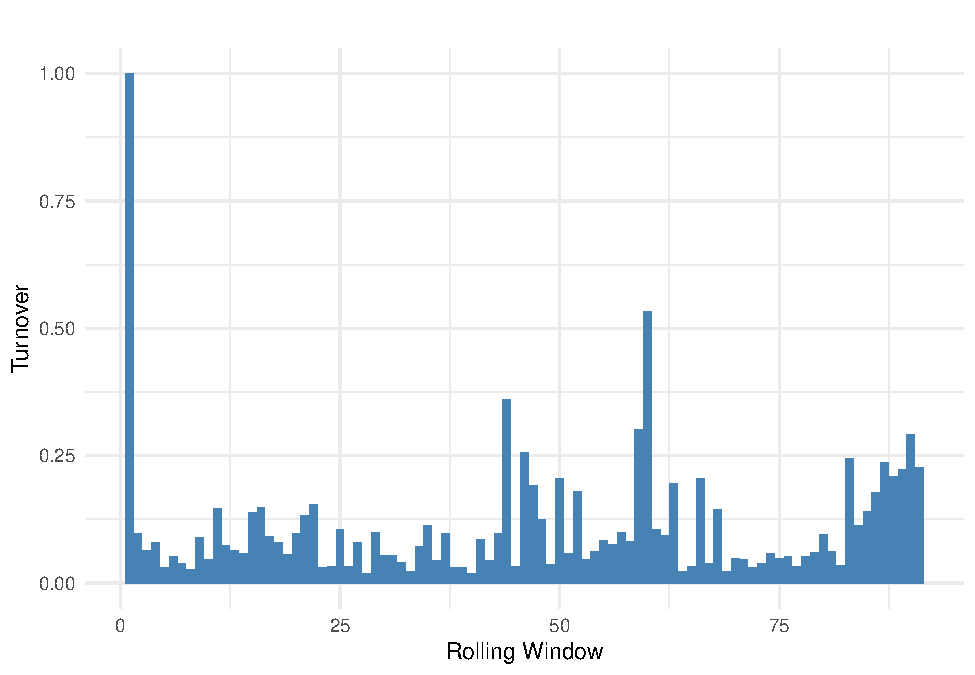
\includegraphics{NDXNES005_A2_RMD_files/figure-latex/unnamed-chunk-8-1.pdf}

\subsubsection{2.8 Jensens alpha and beta}\label{jensens-alpha-and-beta}

\begin{Shaded}
\begin{Highlighting}[]
\CommentTok{\# in{-}sample and out{-}of{-}sample Alpha and Beta}
\NormalTok{ab\_df }\OtherTok{\textless{}{-}} \FunctionTok{data.frame}\NormalTok{(}
  \AttributeTok{Window =} \DecValTok{1}\SpecialCharTok{:}\FunctionTok{length}\NormalTok{(results),}
  \AttributeTok{alpha\_IS =} \FunctionTok{sapply}\NormalTok{(results, }\ControlFlowTok{function}\NormalTok{(x) x}\SpecialCharTok{$}\NormalTok{alpha\_IS),}
  \AttributeTok{alpha\_OOS =} \FunctionTok{sapply}\NormalTok{(results, }\ControlFlowTok{function}\NormalTok{(x) x}\SpecialCharTok{$}\NormalTok{alpha\_OOS),}
  \AttributeTok{beta\_IS =} \FunctionTok{sapply}\NormalTok{(results, }\ControlFlowTok{function}\NormalTok{(x) x}\SpecialCharTok{$}\NormalTok{beta\_IS),}
  \AttributeTok{beta\_OOS =} \FunctionTok{sapply}\NormalTok{(results, }\ControlFlowTok{function}\NormalTok{(x) x}\SpecialCharTok{$}\NormalTok{beta\_OOS)}
\NormalTok{)}

\CommentTok{\# In{-}Sample vs. Out{-}of{-}Sample Jensen\textquotesingle{}s Alpha}
\FunctionTok{ggplot}\NormalTok{(ab\_df, }\FunctionTok{aes}\NormalTok{(}\AttributeTok{x =}\NormalTok{ Window)) }\SpecialCharTok{+}
  \FunctionTok{geom\_line}\NormalTok{(}\FunctionTok{aes}\NormalTok{(}\AttributeTok{y =}\NormalTok{ alpha\_IS, }\AttributeTok{color =} \StringTok{"In{-}Sample"}\NormalTok{), }\AttributeTok{linewidth =} \FloatTok{0.9}\NormalTok{) }\SpecialCharTok{+}
  \FunctionTok{geom\_line}\NormalTok{(}\FunctionTok{aes}\NormalTok{(}\AttributeTok{y =}\NormalTok{ alpha\_OOS, }\AttributeTok{color =} \StringTok{"Out{-}of{-}Sample"}\NormalTok{), }\AttributeTok{linewidth =} \FloatTok{0.9}\NormalTok{) }\SpecialCharTok{+}
  \FunctionTok{labs}\NormalTok{(}\AttributeTok{title =} \StringTok{""}\NormalTok{,}
       \AttributeTok{x =} \StringTok{"Rolling Window"}\NormalTok{, }\AttributeTok{y =} \StringTok{"Alpha"}\NormalTok{, }\AttributeTok{color =} \StringTok{"Sample Type"}\NormalTok{) }\SpecialCharTok{+}
  \FunctionTok{theme\_minimal}\NormalTok{() }\SpecialCharTok{+}
  \FunctionTok{scale\_color\_manual}\NormalTok{(}\AttributeTok{values =} \FunctionTok{c}\NormalTok{(}\StringTok{"In{-}Sample"} \OtherTok{=} \StringTok{"darkgreen"}\NormalTok{, }\StringTok{"Out{-}of{-}Sample"} \OtherTok{=} \StringTok{"darkblue"}\NormalTok{))}
\end{Highlighting}
\end{Shaded}

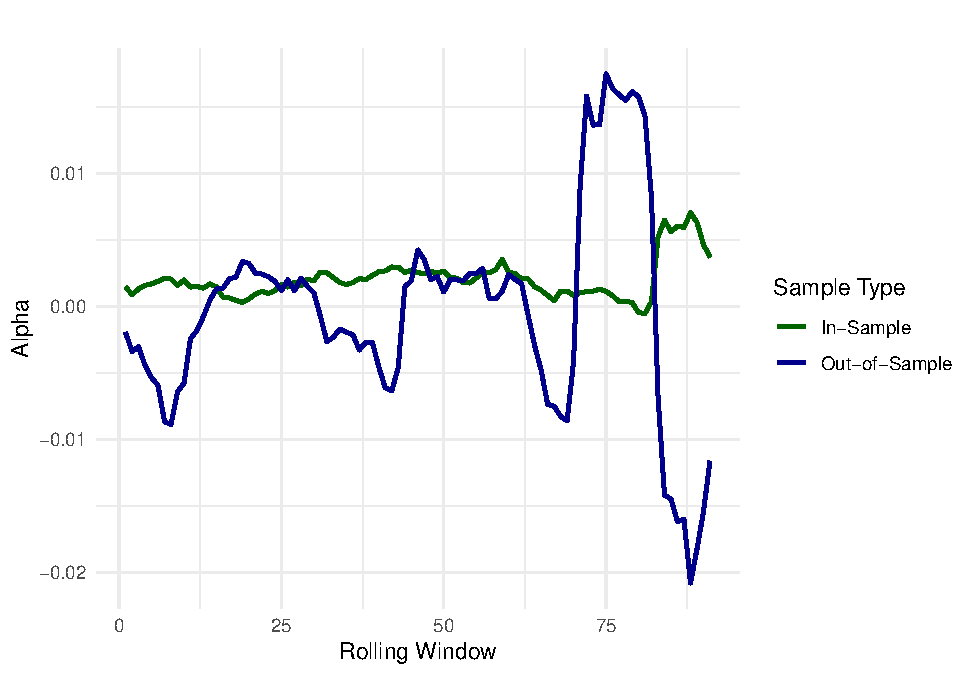
\includegraphics{NDXNES005_A2_RMD_files/figure-latex/unnamed-chunk-9-1.pdf}

\begin{Shaded}
\begin{Highlighting}[]
\CommentTok{\# In{-}Sample vs. Out{-}of{-}Sample Portfolio Beta}
\FunctionTok{ggplot}\NormalTok{(ab\_df, }\FunctionTok{aes}\NormalTok{(}\AttributeTok{x =}\NormalTok{ Window)) }\SpecialCharTok{+}
  \FunctionTok{geom\_line}\NormalTok{(}\FunctionTok{aes}\NormalTok{(}\AttributeTok{y =}\NormalTok{ beta\_IS, }\AttributeTok{color =} \StringTok{"In{-}Sample"}\NormalTok{), }\AttributeTok{linewidth =} \FloatTok{0.9}\NormalTok{) }\SpecialCharTok{+}
  \FunctionTok{geom\_line}\NormalTok{(}\FunctionTok{aes}\NormalTok{(}\AttributeTok{y =}\NormalTok{ beta\_OOS, }\AttributeTok{color =} \StringTok{"Out{-}of{-}Sample"}\NormalTok{), }\AttributeTok{linewidth =} \FloatTok{0.9}\NormalTok{) }\SpecialCharTok{+}
  \FunctionTok{labs}\NormalTok{(}\AttributeTok{title =} \StringTok{""}\NormalTok{,}
       \AttributeTok{x =} \StringTok{"Rolling Window"}\NormalTok{, }\AttributeTok{y =} \StringTok{"Beta"}\NormalTok{, }\AttributeTok{color =} \StringTok{"Sample Type"}\NormalTok{) }\SpecialCharTok{+}
  \FunctionTok{theme\_minimal}\NormalTok{() }\SpecialCharTok{+}
  \FunctionTok{scale\_color\_manual}\NormalTok{(}\AttributeTok{values =} \FunctionTok{c}\NormalTok{(}\StringTok{"In{-}Sample"} \OtherTok{=} \StringTok{"darkred"}\NormalTok{, }\StringTok{"Out{-}of{-}Sample"} \OtherTok{=} \StringTok{"darkorange"}\NormalTok{))}
\end{Highlighting}
\end{Shaded}

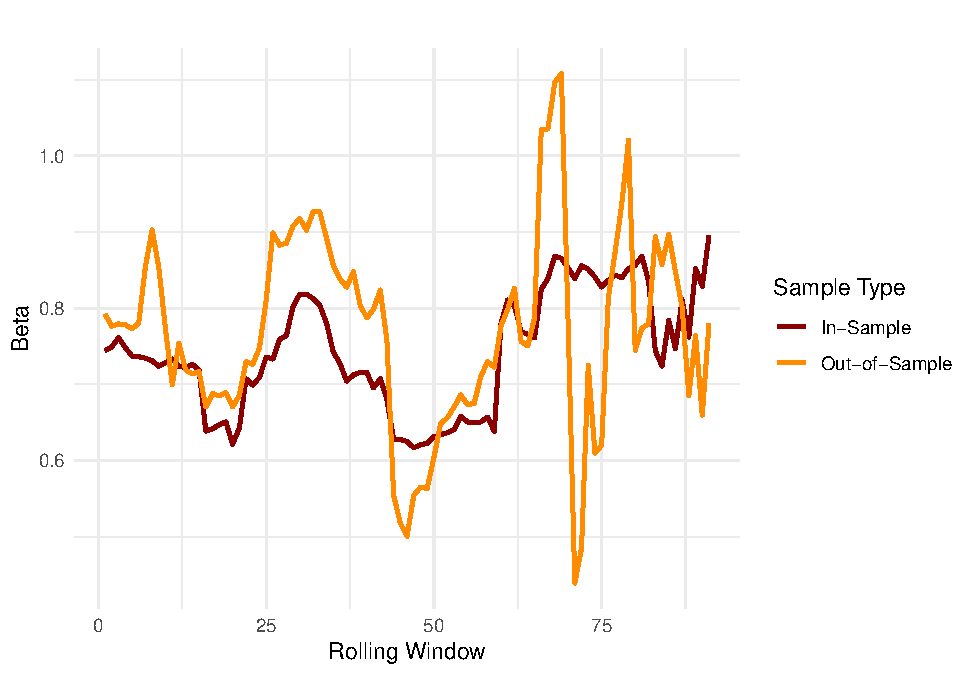
\includegraphics{NDXNES005_A2_RMD_files/figure-latex/unnamed-chunk-9-2.pdf}

\subsubsection{2.9 Plotting In Sample vs Out Of Sample
Statistics}\label{plotting-in-sample-vs-out-of-sample-statistics}

\begin{Shaded}
\begin{Highlighting}[]
\FunctionTok{library}\NormalTok{(tidyr)}
\NormalTok{summary\_df }\OtherTok{\textless{}{-}} \FunctionTok{do.call}\NormalTok{(rbind, }\FunctionTok{lapply}\NormalTok{(}\FunctionTok{seq\_along}\NormalTok{(results), }\ControlFlowTok{function}\NormalTok{(i) \{}
\NormalTok{  x }\OtherTok{\textless{}{-}}\NormalTok{ results[[i]]}
  \FunctionTok{data.frame}\NormalTok{(}
    \AttributeTok{Window =}\NormalTok{ i,  }
    \AttributeTok{train =}\NormalTok{ x}\SpecialCharTok{$}\NormalTok{train\_period,}
    \AttributeTok{test =}\NormalTok{ x}\SpecialCharTok{$}\NormalTok{test\_period,}
    \AttributeTok{mu\_IS =}\NormalTok{ x}\SpecialCharTok{$}\NormalTok{mu\_IS, }\AttributeTok{var\_IS =}\NormalTok{ x}\SpecialCharTok{$}\NormalTok{var\_IS, }\AttributeTok{SR\_IS =}\NormalTok{ x}\SpecialCharTok{$}\NormalTok{SR\_IS,}
    \AttributeTok{mu\_OOS =}\NormalTok{ x}\SpecialCharTok{$}\NormalTok{mu\_OOS, }\AttributeTok{var\_OOS =}\NormalTok{ x}\SpecialCharTok{$}\NormalTok{var\_OOS, }\AttributeTok{SR\_OOS =}\NormalTok{ x}\SpecialCharTok{$}\NormalTok{SR\_OOS,}
    \AttributeTok{alpha\_IS =}\NormalTok{ x}\SpecialCharTok{$}\NormalTok{alpha\_IS, }\AttributeTok{beta\_IS =}\NormalTok{ x}\SpecialCharTok{$}\NormalTok{beta\_IS,}
    \AttributeTok{alpha\_OOS =}\NormalTok{ x}\SpecialCharTok{$}\NormalTok{alpha\_OOS, }\AttributeTok{beta\_OOS =}\NormalTok{ x}\SpecialCharTok{$}\NormalTok{beta\_OOS,}
    \AttributeTok{turnover =}\NormalTok{ x}\SpecialCharTok{$}\NormalTok{turnover,}
    \AttributeTok{t.err =}\NormalTok{ x}\SpecialCharTok{$}\NormalTok{t.err}
\NormalTok{  )}
\NormalTok{\}))}
\NormalTok{sum\_l }\OtherTok{\textless{}{-}}\NormalTok{ summary\_df }\SpecialCharTok{\%\textgreater{}\%}
  \FunctionTok{pivot\_longer}\NormalTok{(}
    \AttributeTok{cols =} \FunctionTok{c}\NormalTok{(mu\_IS, var\_IS, SR\_IS, mu\_OOS, var\_OOS, SR\_OOS),}
    \AttributeTok{names\_to =} \StringTok{"Metric"}\NormalTok{,}
    \AttributeTok{values\_to =} \StringTok{"Value"}
\NormalTok{  ) }\SpecialCharTok{\%\textgreater{}\%}
  \FunctionTok{mutate}\NormalTok{(}
    \AttributeTok{Sample =} \FunctionTok{ifelse}\NormalTok{(}\FunctionTok{grepl}\NormalTok{(}\StringTok{"\_IS"}\NormalTok{, Metric), }\StringTok{"In{-}Sample"}\NormalTok{, }\StringTok{"Out{-}of{-}Sample"}\NormalTok{),}
    \AttributeTok{Metric =} \FunctionTok{gsub}\NormalTok{(}\StringTok{"\_(IS|OOS)"}\NormalTok{, }\StringTok{""}\NormalTok{, Metric),}
    \AttributeTok{Metric =} \FunctionTok{case\_when}\NormalTok{(}
\NormalTok{      Metric }\SpecialCharTok{==} \StringTok{"mu"} \SpecialCharTok{\textasciitilde{}} \StringTok{"Mean"}\NormalTok{,}
\NormalTok{      Metric }\SpecialCharTok{==} \StringTok{"var"} \SpecialCharTok{\textasciitilde{}} \StringTok{"Variance"}\NormalTok{,}
\NormalTok{      Metric }\SpecialCharTok{==} \StringTok{"SR"} \SpecialCharTok{\textasciitilde{}} \StringTok{"Sharpe"}\NormalTok{,}
      \ConstantTok{TRUE} \SpecialCharTok{\textasciitilde{}}\NormalTok{ Metric}
\NormalTok{    )}
\NormalTok{  )}


\CommentTok{\# Mean}
\FunctionTok{ggplot}\NormalTok{(}\FunctionTok{subset}\NormalTok{(sum\_l, Metric }\SpecialCharTok{==} \StringTok{"Mean"}\NormalTok{),}
       \FunctionTok{aes}\NormalTok{(}\AttributeTok{x =}\NormalTok{ Window, }\AttributeTok{y =}\NormalTok{ Value, }\AttributeTok{color =}\NormalTok{ Sample, }\AttributeTok{linetype =}\NormalTok{ Sample)) }\SpecialCharTok{+}
  \FunctionTok{geom\_line}\NormalTok{(}\AttributeTok{linewidth =} \FloatTok{0.9}\NormalTok{) }\SpecialCharTok{+}
  \FunctionTok{labs}\NormalTok{(}
    \AttributeTok{title =} \StringTok{""}\NormalTok{,}
    \AttributeTok{x =} \StringTok{"Rolling Window"}\NormalTok{,}
    \AttributeTok{y =} \StringTok{"Mean Return"}
\NormalTok{  ) }\SpecialCharTok{+}
  \FunctionTok{theme\_minimal}\NormalTok{()}
\end{Highlighting}
\end{Shaded}

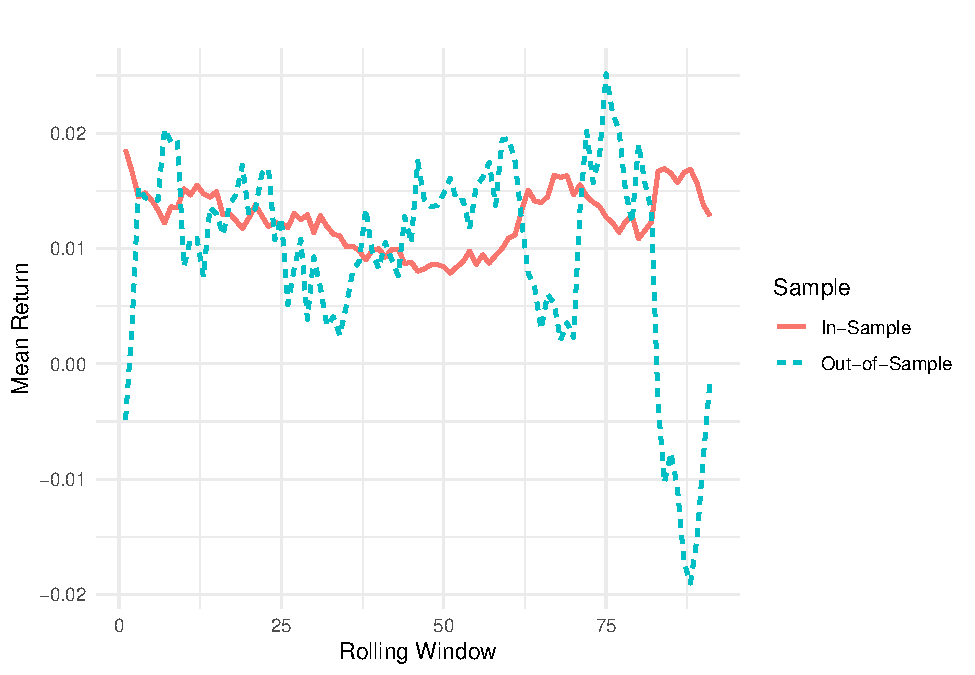
\includegraphics{NDXNES005_A2_RMD_files/figure-latex/unnamed-chunk-10-1.pdf}

\begin{Shaded}
\begin{Highlighting}[]
\CommentTok{\# Variance }
\FunctionTok{ggplot}\NormalTok{(}\FunctionTok{subset}\NormalTok{(sum\_l, Metric }\SpecialCharTok{==} \StringTok{"Variance"}\NormalTok{),}
       \FunctionTok{aes}\NormalTok{(}\AttributeTok{x =}\NormalTok{ Window, }\AttributeTok{y =}\NormalTok{ Value, }\AttributeTok{color =}\NormalTok{ Sample, }\AttributeTok{linetype =}\NormalTok{ Sample)) }\SpecialCharTok{+}
  \FunctionTok{geom\_line}\NormalTok{(}\AttributeTok{linewidth =} \FloatTok{0.9}\NormalTok{) }\SpecialCharTok{+}
  \FunctionTok{labs}\NormalTok{(}
    \AttributeTok{title =} \StringTok{""}\NormalTok{,}
    \AttributeTok{x =} \StringTok{"Rolling Window"}\NormalTok{,}
    \AttributeTok{y =} \StringTok{"Variance"}
\NormalTok{  ) }\SpecialCharTok{+}
  \FunctionTok{theme\_minimal}\NormalTok{()}
\end{Highlighting}
\end{Shaded}

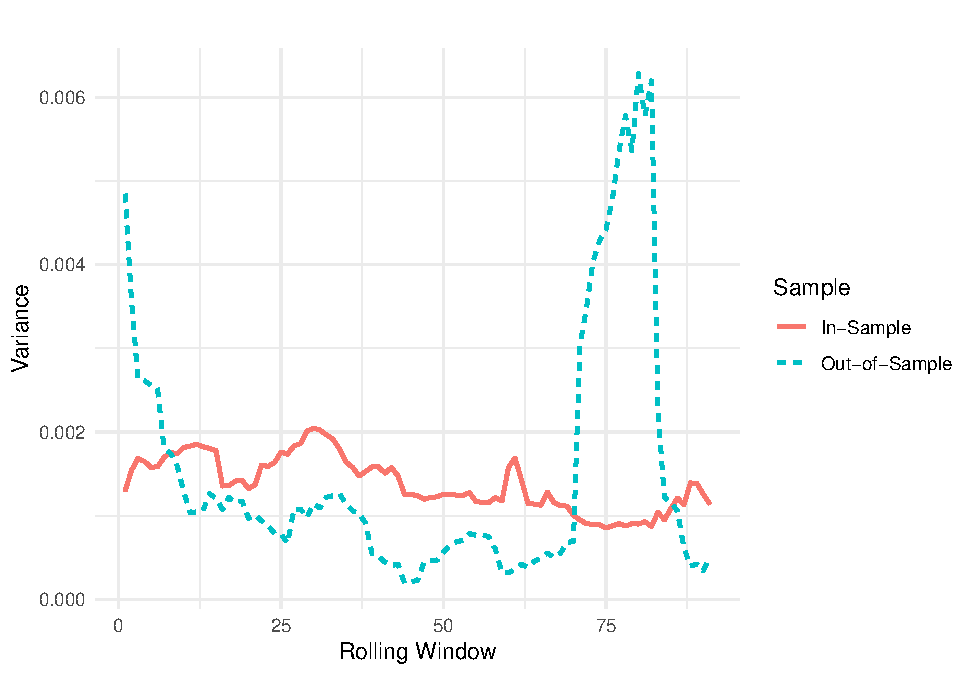
\includegraphics{NDXNES005_A2_RMD_files/figure-latex/unnamed-chunk-10-2.pdf}

\begin{Shaded}
\begin{Highlighting}[]
\CommentTok{\# Sharpe Ratio }
\FunctionTok{ggplot}\NormalTok{(}\FunctionTok{subset}\NormalTok{(sum\_l, Metric }\SpecialCharTok{==} \StringTok{"Sharpe"}\NormalTok{),}
       \FunctionTok{aes}\NormalTok{(}\AttributeTok{x =}\NormalTok{ Window, }\AttributeTok{y =}\NormalTok{ Value, }\AttributeTok{color =}\NormalTok{ Sample, }\AttributeTok{linetype =}\NormalTok{ Sample)) }\SpecialCharTok{+}
  \FunctionTok{geom\_line}\NormalTok{(}\AttributeTok{linewidth =} \FloatTok{0.9}\NormalTok{) }\SpecialCharTok{+}
  \FunctionTok{labs}\NormalTok{(}
    \AttributeTok{title =} \StringTok{""}\NormalTok{,}
    \AttributeTok{x =} \StringTok{"Rolling Window"}\NormalTok{,}
    \AttributeTok{y =} \StringTok{"Sharpe Ratio"}
\NormalTok{  ) }\SpecialCharTok{+}
  \FunctionTok{theme\_minimal}\NormalTok{()}
\end{Highlighting}
\end{Shaded}

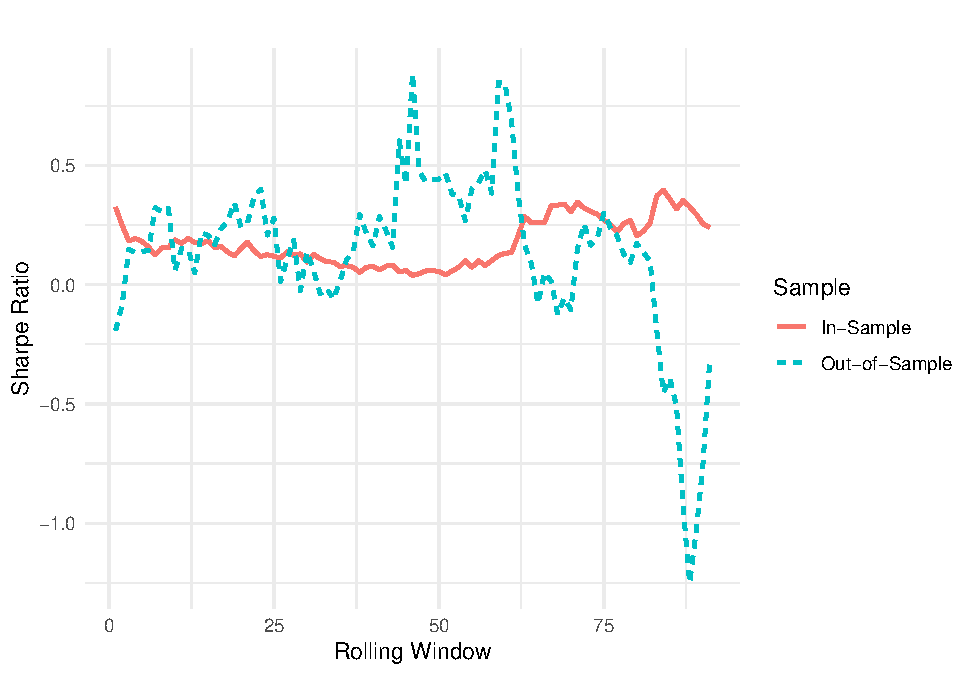
\includegraphics{NDXNES005_A2_RMD_files/figure-latex/unnamed-chunk-10-3.pdf}

\subsubsection{2.10 Portfolio Weights}\label{portfolio-weights}

\begin{Shaded}
\begin{Highlighting}[]
\CommentTok{\# Combine all rolling window weights into a single data frame}
\NormalTok{weights\_df }\OtherTok{\textless{}{-}} \FunctionTok{do.call}\NormalTok{(rbind, }\FunctionTok{lapply}\NormalTok{(}\FunctionTok{seq\_along}\NormalTok{(results), }\ControlFlowTok{function}\NormalTok{(i) \{}
  \FunctionTok{data.frame}\NormalTok{(}
    \AttributeTok{Window =}\NormalTok{ i, }\CommentTok{\#index}
    \AttributeTok{Asset  =}\NormalTok{ results[[i]]}\SpecialCharTok{$}\NormalTok{assets,}\CommentTok{\# asset names}
    \AttributeTok{Weight =}\NormalTok{ results[[i]]}\SpecialCharTok{$}\NormalTok{weights,}\CommentTok{\#  weights}
    \AttributeTok{stringsAsFactors =} \ConstantTok{FALSE}
\NormalTok{  )}
\NormalTok{\}))}

\CommentTok{\# Evolution of Black{-}Litterman Portfolio Weights}
\FunctionTok{ggplot}\NormalTok{(weights\_df, }\FunctionTok{aes}\NormalTok{(}\AttributeTok{x =}\NormalTok{ Window, }\AttributeTok{y =}\NormalTok{ Asset, }\AttributeTok{fill =}\NormalTok{ Weight)) }\SpecialCharTok{+}
  \FunctionTok{geom\_tile}\NormalTok{(}\AttributeTok{color =} \StringTok{"white"}\NormalTok{) }\SpecialCharTok{+}
  \FunctionTok{scale\_fill\_gradient}\NormalTok{(}\AttributeTok{low =} \StringTok{"white"}\NormalTok{, }\AttributeTok{high =} \StringTok{"steelblue"}\NormalTok{) }\SpecialCharTok{+}
  \FunctionTok{scale\_x\_continuous}\NormalTok{(}
    \AttributeTok{breaks =} \FunctionTok{seq}\NormalTok{(}\FunctionTok{min}\NormalTok{(weights\_df}\SpecialCharTok{$}\NormalTok{Window), }\FunctionTok{max}\NormalTok{(weights\_df}\SpecialCharTok{$}\NormalTok{Window), }\AttributeTok{by =} \DecValTok{5}\NormalTok{)}
\NormalTok{  ) }\SpecialCharTok{+}
  \FunctionTok{labs}\NormalTok{(}
    \AttributeTok{title =} \StringTok{""}\NormalTok{,}
    \AttributeTok{x =} \StringTok{"Rolling Window Index"}\NormalTok{,}
    \AttributeTok{y =} \StringTok{"Asset"}\NormalTok{,}
    \AttributeTok{fill =} \StringTok{"Weight"}
\NormalTok{  ) }\SpecialCharTok{+}
  \FunctionTok{theme\_minimal}\NormalTok{() }\SpecialCharTok{+}
  \FunctionTok{theme}\NormalTok{(}\AttributeTok{axis.text.x =} \FunctionTok{element\_text}\NormalTok{(}\AttributeTok{angle =} \DecValTok{45}\NormalTok{, }\AttributeTok{hjust =} \DecValTok{1}\NormalTok{))}
\end{Highlighting}
\end{Shaded}

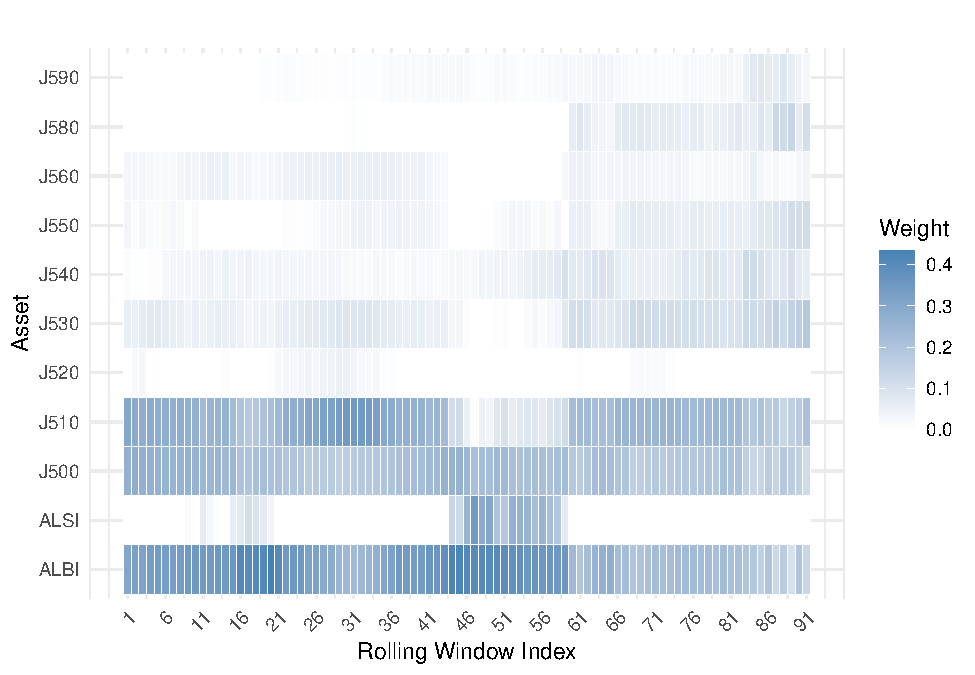
\includegraphics{NDXNES005_A2_RMD_files/figure-latex/unnamed-chunk-11-1.pdf}

\subsubsection{2.11 Tracking Error}\label{tracking-error}

\begin{Shaded}
\begin{Highlighting}[]
\DocumentationTok{\#\#\# Tracking Error Plot}
\NormalTok{t.err\_df }\OtherTok{\textless{}{-}} \FunctionTok{data.frame}\NormalTok{(}
  \AttributeTok{Window =} \DecValTok{1}\SpecialCharTok{:}\FunctionTok{length}\NormalTok{(results),}
  \AttributeTok{TrackingError =} \FunctionTok{sapply}\NormalTok{(results, }\ControlFlowTok{function}\NormalTok{(x) x}\SpecialCharTok{$}\NormalTok{t.err)}
\NormalTok{)}
\CommentTok{\# Rolling Window Tracking Error vs ALSI}
\FunctionTok{ggplot}\NormalTok{(t.err\_df, }\FunctionTok{aes}\NormalTok{(}\AttributeTok{x =}\NormalTok{ Window, }\AttributeTok{y =}\NormalTok{ TrackingError)) }\SpecialCharTok{+}
  \FunctionTok{geom\_line}\NormalTok{(}\AttributeTok{linewidth =} \FloatTok{0.9}\NormalTok{) }\SpecialCharTok{+}
  \FunctionTok{geom\_hline}\NormalTok{(}\AttributeTok{yintercept =} \FloatTok{0.03}\NormalTok{, }\AttributeTok{linetype=}\StringTok{"dashed"}\NormalTok{) }\SpecialCharTok{+}
  \FunctionTok{geom\_hline}\NormalTok{(}\AttributeTok{yintercept =} \FloatTok{0.10}\NormalTok{, }\AttributeTok{linetype=}\StringTok{"dashed"}\NormalTok{) }\SpecialCharTok{+}
  \FunctionTok{labs}\NormalTok{(}\AttributeTok{title =} \StringTok{""}\NormalTok{,}
       \AttributeTok{x =} \StringTok{"Rolling Window"}\NormalTok{, }\AttributeTok{y =} \StringTok{"Tracking Error"}\NormalTok{) }\SpecialCharTok{+}
  \FunctionTok{theme\_minimal}\NormalTok{()}
\end{Highlighting}
\end{Shaded}

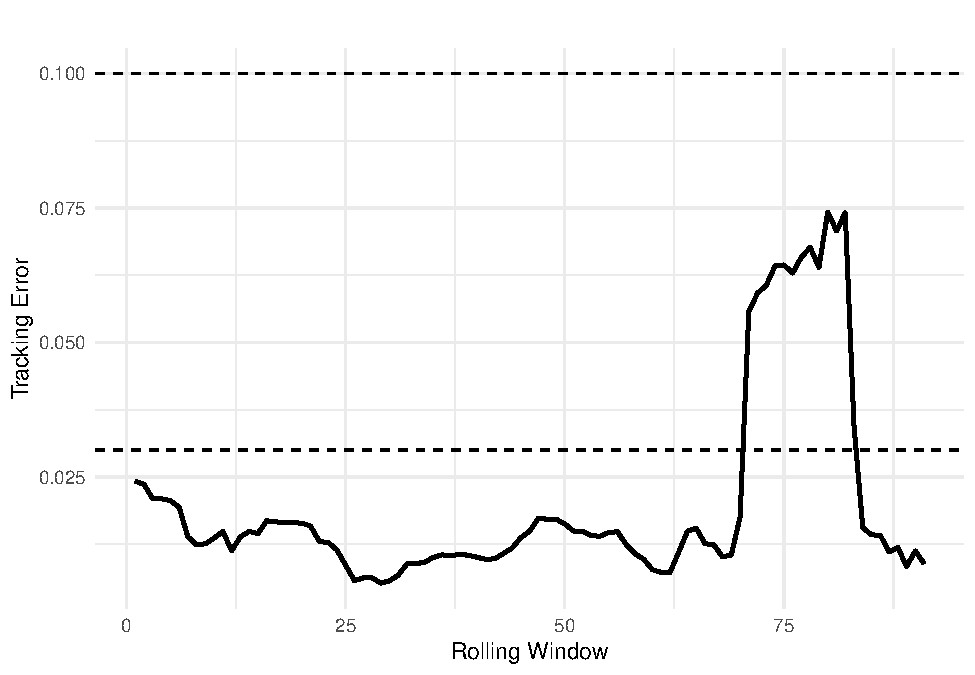
\includegraphics{NDXNES005_A2_RMD_files/figure-latex/unnamed-chunk-12-1.pdf}

\newpage

\section*{References}\label{references}
\addcontentsline{toc}{section}{References}

\phantomsection\label{refs}
\begin{CSLReferences}{1}{0}
\bibitem[\citeproctext]{ref-Tim_BT}
Gebbie, T. (2025a). \emph{PortfolioTheory-backtest-001.r}. Unpublished
teaching material.

\bibitem[\citeproctext]{ref-Tim_prepmlx}
Gebbie, T. (2025b). \emph{PortfolioTheoryLecture001.mlx}. Unpublished
teaching material.

\bibitem[\citeproctext]{ref-Tim_BTmlx}
Gebbie, T. (2025c). \emph{PortfolioTheoryLecture003.pdf}. Unpublished
teaching material.

\bibitem[\citeproctext]{ref-Tim_prep}
Gebbie, T. (2025d). \emph{PortfolioTheory-PrepareData-000.r}.
Unpublished teaching material.

\end{CSLReferences}

\end{document}
